\chapter{Atmosférické srážky a metody měření\\jejich objemu}
\subsubsection{Co to jsou srážky?}
    Pojmem srážky se rozumí veškerá voda v atmosféře v jakémkoliv skupenství. Srážky rozdělujeme na padající, usazené a takzvanou virgu — suché srážky, srážkové pruhy. Za padající srážky označujeme všechny formy vody padající z atmosféry na zemský povrch, z této kategorie můžeme jmenovat například déšť, kroupy a sníh. Za srážky usazené považujeme vodu ležící na zemském povrchu — rosu, jinovatku.  Srážky označené jako virga jsou definovány jako srážky, které sice vypadávají z mraku, ale z různých důvodů již nedopadnou na zem \cite{eunxinImJJLla7m6}. Stanovení intenzity srážek nemá žádný vědecký podklad, ale pomocně si intenzitu můžeme rozdělit do jednoduché tabulky  \ref{table:rozděleníSrážek}.
    
    \begin{table}[!h]
      \caption[Rozdělení srážek]{Rozdělení intenzity srážek na základě hodinového úhrnu.}
      \label{table:rozděleníSrážek}
      \begin{center}
      	\small
    	  \begin{tabular}{|c|c|}
    	    \hline
    	    Intenzita srážek & Úhrn srážek [mm/h]\\
    	    \hline\hline
    	    Velmi slabá & <1 \\
    	    \hline
    	    Slabá & 1 — 2  \\
    	    \hline
    	    Mírná & 2 — 8  \\
    	    \hline
    	    Silná & 8 — 40  \\
    	    \hline
    	    Velmi silná & >40  \\
    	    \hline
    	  \end{tabular}
      \end{center}
    \end{table}
    
\subsubsection{Důvody měření srážek}
    Informace o objemu spadlých srážek na určitém území můžeme využít v nejrůznějších oblastech. V zemědělství pro predikci vhodného období pro setbu či sklizeň. Ve stavebním inženýrství využíváme tyto informace k plánování částí staveb nebo k dimenzování odtoků vody z komunikací. V hydrometeorologických ústavech pro výzkum či vydávání výstražných informací \cite{wR7t0M6HVRhIssnr}.
    
\section{Techniky měření srážek}
    Srážky se měří zařízením zvaným srážkoměr. V nejjednodušší podobě se jedná o válcovitou nádobu, jenž je umístěna na vodorovné ploše, daleko od všech možných překážek jako například budovy či stromy, které by mohli bránit sběru srážek při nepříznivých podmínkách. K zamezení ovlivnění měření srážek stíněním srážkoměru se doporučuje umístit srážkoměr do minimálně dvojnásobné výšky okolních překážek. Srážkoměry můžeme dělit na ručně obsluhované a automatizované \cite{nkURfCvWR2piX49C}.

\subsection{Ručně obsluhované srážkoměry}
    \par Manuální srážkoměry jsou nejčastěji objemově cejchované nádoby, ke kterým musí denně obsluha v určitý čas přijít a odečtený objem srážek zapsat manuálně do deníku či do počítačového programu. 
    \par Tyto srážkoměry mají pouze omezený objem a nemohou se samy vylévat, je zde tudíž nutnost kontrolovat objem srážek a v případě velmi velkého úhrnu je nutné provádět odečty i vícekrát denně. Další možností je použití necejchované nádoby, kde se k měření využívá cejchovaná odměrka, do které je objem nádoby pokaždé přelit. U této možnosti je možné do měření zanést chybu v případě kdy nedojde k celému vyprázdnění sběrné nádoby do odměrky. Další možnou chybou při manuálním měření srážek je špatný odečet objemu. I přes zmíněné možnosti chyb se jedná o nejpřesnější metodu měření úhrnu srážek. V případě tuhých srážek je jejich objem rozehřát a srážky jsou měřeny v kapalném skupenství. V dnešní době se na řadě míst ručně obsluhované srážkoměry vyměňují za automatizované měřicí stanice ať už z důvodu špatné dostupnosti či nedostatkem personálu \cite{nkURfCvWR2piX49C, ggXzrltWxOZUtGvb}.
    \par Ve špatně dostupném terénu se můžeme setkat s tzv. totalizátory, ze kterých se objemy srážek vyčítají zpravidla každý půl rok (zpravidla na jaře a na podzim z důvodu odlišení tuhých a kapalných srážek). Jedná se o srážkoměr o záchytné ploše 200 cm$^2$ ve výšce 3 až 5 metrů nad okolním terénem. Objem záchytné nádrže musí být dostatečně velký se zohledněním délky měření a předpokládaným objemem srážek, jeho objem se může pohybovat i ve stovkách litrů. Do záchytné nádrže se umisťuje olej, který zabraňuje výparu, v zimních měsících se do nádrže doplňuje nemrznoucí roztok (nejčastěji chlorid vápenatý). V České republice je momentálně provozováno 24 totalizátorů umístěných povětšinou na hřebenech hor \cite{gg4G3GDssPMW65VW, gsSBFoB7VG748RwB, PhmBl0LI513CX5w2}.
    \par Typické vnitřní uspořádání manuálního srážkoměru je vyobrazeno na obrázku \ref{obr:Srážkoměr}.

    \begin{figure}[!h]
      \begin{center}
        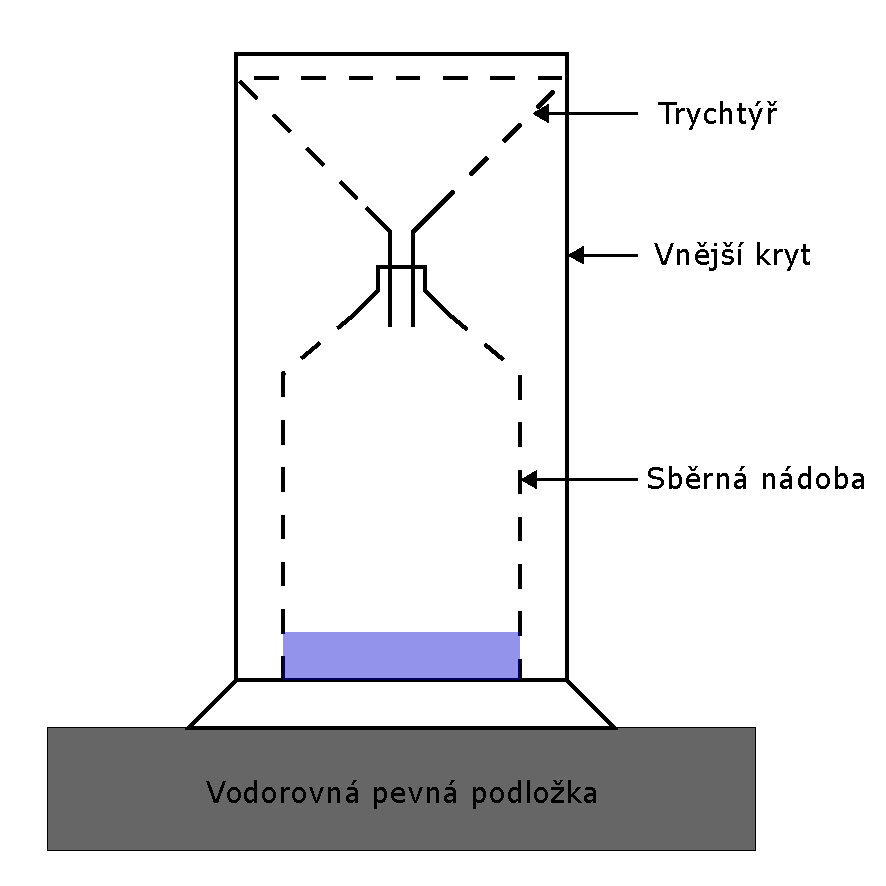
\includegraphics[scale=0.7]{obrazky/prace/rain_gauge.pdf}
      \end{center}
      \caption[Srážkoměr]{Nákres nejjednodušší formy srážkoměru \cite{nkURfCvWR2piX49C}}
      \label{obr:Srážkoměr}
    \end{figure}

\subsection{Člunkový srážkoměr}
\par Člunkový srážkoměr je tvořen trychtýřem, jehož ústí je umístěno nad překlápěcím člunkem. Pokud je jedna část člunku naplněna přesně definovaným objemem vody dojde k jeho překlopení. V momentě tohoto překlopení dojde k zaznamenání této události a k vylití vody z této poloviny. Srážky jsou v tento moment svedeny do druhé poloviny. Po naplnění druhé poloviny se celý proces opakuje. Vnitřní uspořádání člunkového srážkoměru je naznačeno na obrázku \ref{obr:tipping_bucket}. Vylévaná voda může být sbírána do nádoby k pozdějšímu validování dat. Pro měření tuhých srážek může být zařízení doplněno vyhříváním \cite{nkURfCvWR2piX49C}.
\par Tento typ srážkoměru je v případě dobrého umístění značně bezúdržbový, hrozí zde pouze zanesení trychtýře a mechanismu nečistotami, v případě plastových srážkoměrů nemůžeme vyloučit poškození například většími kroupami.
\par Při měření je možný výskyt několika druhů chyb. Pokud objem srážek není dostatečný k překlopení člunku srážkoměru, může nastat chyba nezaznamenání srážek, případná nahromaděná kapalina může ovlivnit měření následujících srážek. Další chyba může nastat u velmi rychlého a velmi velkého srážkového úhrnu, kdy může dojít k přetečení člunku či zahlcení záznamového zařízení \cite{ggXzrltWxOZUtGvb, Lewlomphaisarl}.
\par I když tento typ srážkoměru nepatří mezi nejpřesnější jeho největší výhoda je extrémně nízká spotřeba energie, je tedy hojně využíván u všech projektů pracujícími s omezenou dostupností energie. Vzhledem k nízké ceně a dostačující přesnosti pro většinu použití je také dodáván k většině komerčních meteostanic.
    \begin{figure}[!h]
      \begin{center}
        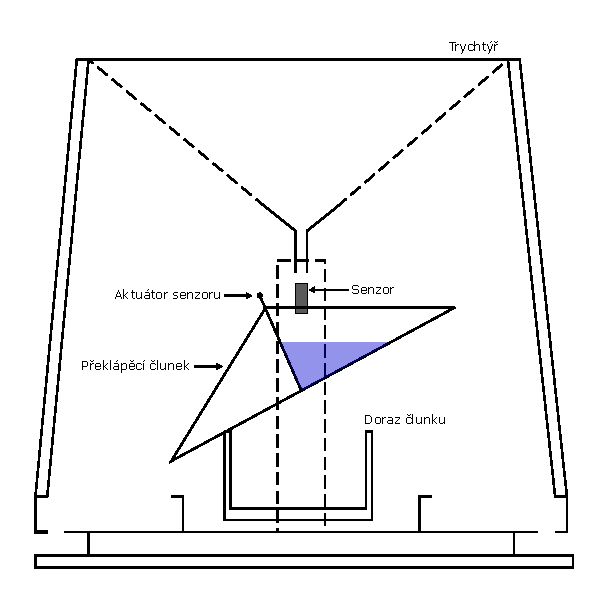
\includegraphics[scale=1]{obrazky/prace/tipping_bucket.pdf}
      \end{center}
      \caption[Člunkový srážkoměr]{Nákres člunkového srážkoměru \cite{Lewlomphaisarl}}
      \label{obr:tipping_bucket}
    \end{figure}

\subsection{Srážkoměr s váhovým senzorem}
\par Tento typ srážkoměru je jedním z novějších metod měření srážek vyvinutém v roce 1992 slovenskou společností MPS Systems. Jeho funkce je založena na měření váhových příbytků v čase. Díky tomuto způsobu měření můžeme při velmi rychlém záznamu dat tento typ srážkoměru využít k velmi přesnému záznamu aktuálního úhrnu srážek \cite{ggXzrltWxOZUtGvb}.
\par Výpusť sběrného trychtýře je umístěna nad sběrnou nádobou, která leží na váhových (například tenzometrických) senzorech. Můžeme se také setkat se samo vyprazdňovací funkcí, tyto srážkoměry poté fungují na podobném principu jako člunkový typ, kde člunkový mechanismus je umístěn na váhovém senzoru. Výhodou tohoto řešení je odstranění chyby způsobené nedostatečným objemem spadlých srážek nutným pro překlopení srážkoměru, jelikož aktuální úhrn můžeme zaznamenat váhovým rozdílem \cite{ggXzrltWxOZUtGvb}. 
\par Srážkoměry s váhovými senzory jsou nejčastěji využívány meteorologickými společnostmi, jelikož jsou často velmi nákladná (nejen srážkoměry samotné, ale také zpracování dat, které vyžadují nejen nepřetržitý záznam ale také značné následné zpracování) a vyžadují častou údržbu z důvodu produkce chyb v případě zanesení srážkoměru nečistotami jejichž váha se přičítá k váze měřené kapalin. Další chybu způsobuje vypařování kapaliny v nádobě, tento problém se dá zmírnit malým množstvím oleje, který se drží nad vodou a zabraňuje jejímu vypařování. Srážkoměry jsou také náchylné k otřesům, které produkuje například silný vítr \cite{ggXzrltWxOZUtGvb}.

\subsection{Další způsoby měření srážek}

\subsubsection{Radarové odhady srážek}
\par Všechny typy pozemních srážkoměrů mají jednu stejnou nevýhodu, a to že měření probíhá pouze na jednom určeném místě. Pro měření srážek plošně pro větší území využíváme radarové odhady. 
Radarové odhady pracují s výkonem odraženého signálu od srážek. Dle tohoto výkonu dokážeme matematicky identifikovat druh srážek a jejich vzdálenost k radaru. Pro určení srážkové intenzity se využívá závislosti radarového odrazu a určené intenzity \cite{6eWEbsB9cSdSJAFB, Salek2012}.
\par V České republice provozuje dva meteorologické radary Český hydrometeorologický ústav. První radar se nachází ve středních Čechách na vrchu Praha v Brdech, pracuje s frekvencí 5630 MHz o výkonu 250 kW a je schopen detekovat srážky v maximální vzdálenosti 260 km. Druhý radar se nachází na střední Moravě na vrchu Skalky u obce Protivanov, pracuje na frekvenci 5645 MHz, ostatní parametry jsou stejné jako u radaru v Brdech \cite{KUiFYNNRR6FRo4R1}.

\subsubsection{Oportunistické metody — měření srážek pomocí mikrovlnných spojů}
\par Komerční mikrovlnné spoje, ve většině případů využívající frekvence 5 a 40 GHz, pro svou funkčnost spoléhají na přímou viditelnost mezi základovými stanicemi. Srážkové odhady založené na faktu, že srážky procházející mezi těmito základovými stanicemi, měřitelně utlumí všechny signály jimi procházející tak jak je naznačeno na obrázku \ref{obr:CML}, zvláště potom ty jejichž frekvence přesahuje 15 GHz. Odhad srážkového úhrnu pomocí mikrovlnného spoje se dá vypočítat pomocí jednoduché rovnice $k=a*R^{2}$ kde $k$ představuje útlum způsobený srážkami v dB/km a $R$ představuje srážkový úhrn v mm/hodina, parametry $a$ a $b$ jsou  závislé na frekvenci a polarizaci mikrovlnného spoje. Po získání potřebných dat, které nejsou žádným způsobem standardizována, přichází hlavní problém, a to identifikace útlumu způsobeného srážkami \cite{Chwala2019, Bubniak20221011}. 

    \begin{figure}[!h]
      \begin{center}
        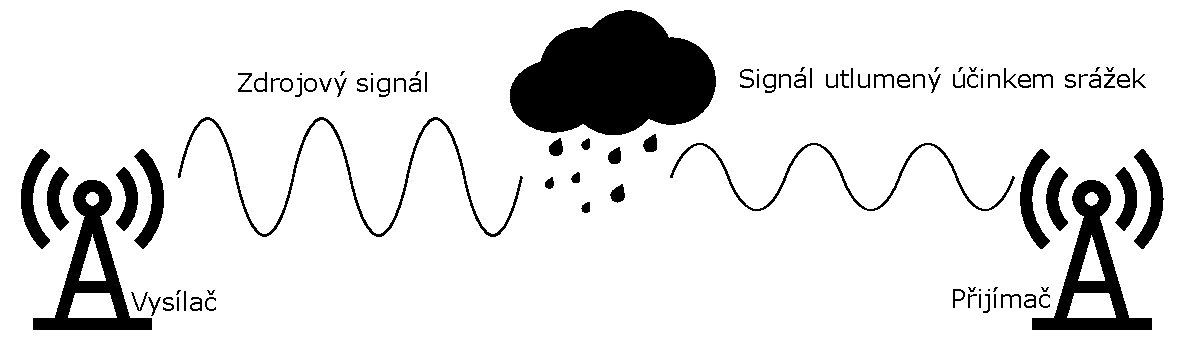
\includegraphics[scale=0.5]{obrazky/prace/cml.pdf}
      \end{center}
      \caption[CML]{Základní princip měření úhrnu srážek pomocí mikrovlnných spojů \cite{Chwala2019}}
      \label{obr:CML}
    \end{figure}
    
\par Pro zpracování dat získaných z mikrovlnných spojů můžeme zveřejněné knihovny RAINLINK\footnote{RAINLINK dostupný z: \url{https://github.com/overeem11/RAINLINK}} určené pro programovací jazyk R, opensource knihovny pycomlink\footnote{pycomlink dostupný z: \url{https://github.com/pycomlink/pycomlink}} v programovacím jazyce python, případně grafického programu Telcorain\footnote{Telcorain dostupný z: \url{https://github.com/milbub/Telcorain}} vyvíjeného na půdě Fakulty elektrotechniky a komunikačních technologií VUT v Brně \cite{Chwala2019, Bubniak20221011}.

\chapter{Internet věcí}
\par Internet věcí (Internet of Things, IoT) je pojem užívaný pro všechna adresovatelná fyzická zařízení, která si mezi sebou předávají data. Tato komunikace probíhá na úrovni zařízení — zařízení (Machine to Machine, M2M), tedy bez lidského přičinění. Věcí je označován jakýkoliv prvek, kterému může být přiřazena IP adresa a může přes síť odesílat data. Toto věc je tvořena třemi základními prvky: senzorem nebo akčním členem, procesorem a komunikátorem. Senzor interaguje s okolím a měří různé fyzikální veličiny jako například teplotu, sílu magnetického pole, elektrické napětí atd. Případný akční člen vykonává dle typu určitou práci. Procesor komunikuje se senzorem či akčním členem a zpracovává naměřená data nebo zpracovává přijaté příkazy. Zpracovaná data procesor dále předá komunikačnímu modulu, který je po komunikační síti pošle dále. Tyto data přijme další zařízení, které je může převést z jedné komunikační sítě na druhou (gateway) nebo data přijme a dále zpracuje (server) \cite{Gillisc20052022}. 

\section{Low-power wide-area networks}
\par Možností, jak zařízení připojit do internetu věcí je celá řada. Připojení může být drátové pomocí Ethernetu nebo bezdrátové například pomocí WiFi. U celé řady zařízení je ale nutné, aby komunikace byla možná na dlouhou vzdálenost, a přitom s malým výkonem z důvodu dlouhé výdrže baterií. Pro tyto zařízení byla definována Low-Power Wide-Area Network (LPWAN). Vlastnosti, jež definují LPWAN jsou: 
\begin{itemize}
    \item Malý výkon — velmi malá spotřeba energie, umožňuje nasazení koncových zařízení s velmi dlouhou, téměř doživotní, výdrží baterie.
    \item Dlouhý dosah — dosah koncových zařízení v otevřeném prostoru se může pohybovat v desítkách kilometrů.
    \item Nízká cena — jednoduchost LPWAN technologií se odráží v koncové cenně koncových zařízení, umožňuje velmi rychlý nárůst počtu nasazených zařízení.
\end{itemize}
Vlastnosti nejrozšířenějších LPWAN technologií jako \acs{LoRa}, Sigfox a Narrowband-IoT porovnáváme v tabulce \ref{table:rozděleníLPWAN} \cite{fadsYdeDtJIDXq0T}.

\begin{table}[!h]
\caption[Vlastnosti LPWAN technologií]{Vlastnosti nejrozšířenějších LPWAN technologií \cite{J76NlDAVQuEhT6co, B5fEKVY7u8J8dyUq, Stusek2019}}
\label{table:rozděleníLPWAN}
\begin{center}
\small
\begin{tabular}{|p{3cm}|p{3cm}|p{3cm}|p{3cm}|}
\hline
& \acs{LoRaWAN} & Sigfox & \acs{NB-IoT}\\
\hline \hline
Dosah & 40 km & 40 km & 20 km\\
\hline
Technologie & Proprietární & Proprietární & \acs{LTE}\\
\hline
Frekvenční pásmo & Bezlicenční \acs{ISM} & Bezlicenční \acs{ISM} & Licenční\\
\hline
Omezení střídy & Ano (1\%) & Ano (1\%) & Ne\\
\hline
Vysílací výkon & 14 dBm = 25 mW (Omezeno) & 14 dBm = 25 mW (Omezeno) & 23 dBm = 200 mW\\
\hline
Datová rychlost & 10 kb/s & 100 b/s & 200 kb/s\\
\hline
Maximální velikost zprávy & 243 B & 12 B (\acs{UL}), 8 B (\acs{DL}) & 1280 B\\
\hline
Doba provozu & 10+ let & 10+ let & 10+ let\\
\hline
\end{tabular}
\end{center}
\end{table}


\subsection{\acs{LoRa}}
\par LoRa odvozena od "Long Range" je proprietární modulační technika vyvinuta společností Cycleo, dnes patřící pod společnost Semtech. Modulační technika \acs{LoRa} pracuje s rozprostřeným spektrem díky čemuž může pracovat se signály na prahu šumu. Pro každou datovou rychlost je odvozena šířka pásma a faktor rozprostření. Díky odstupňování datových rychlostí můžeme volit mezi přenosovou rychlostí a přenosovou vzdáleností na základě koncové aplikace. Signál modulovaný \acs{LoRa} technikou je určen pro přenos rádiovým signálem pomocí protokolu \acs{LoRaWAN} \cite{B5fEKVY7u8J8dyUq, Pech2019}.
\par Zařízení pracující s protokolem \acs{LoRaWAN} využívají k přenosu bezlicenčních \acs{ISM} pásem určených k průmyslovému a vědeckému použití. V Evropě se nejčastěji využívají kmitočty 433 a 868 MHz. Rádiová komunikace na bezlicenčním pásmu není nijak zpoplatněna, ale je omezena střídou vysílání, které činní 1 \% času. \acs{LoRaWAN} se touto omezení vyhýbá vysíláním na více kanálech. Sítě postavené na \acs{LoRaWAN} mají ve většině řešení topologii hvězdy, v jejímž středu se nachází brána (gateway) jež převádí rádiový signál na IP. Můžeme ale realizovat i peer to peer (P2P) spojení mezi jednotlivými zařízeními. Pro přenášení dat můžeme využít vlastní infrastruktury, využít komerčních bran (v ČR tuto službu poskytují například České Radiokomunikace) nebo se můžeme zapojit do komunitních sítí (kupříkladu projekt The Things Network), které propojují brány v soukromém vlastnictví do jednoho celku \cite{B5fEKVY7u8J8dyUq, Pech2019}. 
\par Společnost Semtech udává dosah signálu modulovaného pomocí LoRy až 30 mil v otevřeném prostoru, ale v rámci pokoření světového rekordu byla pokořena vzdálenost přesahující 730 tisíc kilometrů, kdy se podařilo rádiový signál odrazit od povrchu měsíce. V případě nedostupnosti signálu v plánované oblasti nasazení zařízení, můžeme taky uvažovat nad využitím satelitních opakovačů. Takovouto službu nabízí například společnost Fossa systems \cite{b2bXQAhEG5l7OcrW, jP0mkWtryNxDkAWP}. 

\subsection{Sigfox}
\par Sigfox je LPWA komunikační protokol a LPWAN síť pracující v bezlicenčním \acs{ISM} pásmu na frekvencích 868 MHz v Evropě a 915 MHz v Americe. Stejně jako \acs{LoRaWAN} je Sigfox budován v topologii hvězda, v jejímž středu je brána. Na rozdíl od LoRaWANu brány nepřeposílají data na koncový server nýbrž Sigfox cloudu.  I když Sigfox využívá bezlicenčního pásma je přenos dat po této síti zpoplatněn. Provozovatelem Sigfoxu v České republice je společnost Sigfox Česká republika (dříve SimpleCell Networks), která společně s operátorem T-Mobile buduje síť bran na našem území. Cena tarifu je odvozena od množství \acs{UL} a \acs{DL} zpráv. Nejvyšší tarif nabízí 140 \acs{UL} zpráv denně s maximálně 12 bajty na zprávu. Pokud chceme zasílat data směrem do zařízení jsme limitováni 4 zprávami denně s maximální velikostí 8 bajtů na každou zprávu \cite{FM8jojRfULuDpOXz}.
\par Vzhledem k závislosti Sigfoxu na cloudu vznikají pochybnosti o jejím využití v budoucích projektech, zvláště poté co společnost Sigfox čelila úpadku a v lednu roku 2022 požádala o soudní ochranu, zatímco se pokouší najít kupce. V březnu téže roku společnost oznámila její akvizici společností UnaBiz Technology \cite{Sedlak3112022, Swinhoe23032022}.

\subsection{Narrowband-IoT}
\par Technologie narrowband-IoT (NB-IoT) byla představena jako odpověď telekomunikačních operátorů na sítě \acs{LoRaWAN} a Sigfox. První \acs{NB-IoT} standart představila iniciativa Third Generation Partnership Project (3GPP) v roce 2016 ve 13. vydání s oficiálním názvem \acs{LTE} cat NB1. Jedná se o technologii pro přenos dat v internetu věcí po stávajících licencovaných pásmech s využitím technické infrastruktury a fyzické vrstvy technologie LTE. Díky využití \acs{LTE} infrastruktury v sítích \acs{NB-IoT} je nasazení koncových aplikací značně urychleno v kontrastu sítí \acs{LoRaWAN} a Sigfox jenž vyžadují vybudování nové infrastruktury \cite{Mozny2019, tBSoZdNaMrfO37cI, Pech20192, K5NubB0NtDsrG3dJ}. 

\subsubsection{Fyzická vrstva NB-IoT}
\par Jak už slovo "narrowband" v názvu technologie napovídá, systém využívá úzkou šířku pásma a to konkrétně 180 kHz. Tato šířka pásma odpovídá jednomu zdrojovému bloku \acs{LTE}, kde zdrojový blok je nejmenší jednotka zdrojů, které mohou být přiděleny jednomu zařízení. Pro \acs{NB-IoT} jsou specifikovány tři operační módy: standalone, guard-band a in-band \cite{Schlienz882016}.
    \begin{itemize}
        \item Standalone mód: v tomto módu \acs{NB-IoT} využívá frekvenčních pásem využívaných technologií Global System for Mobile Communications (GSM) jehož bloky využívají 200 kHz šířku pásma. Pokud tento blok využijeme pro \acs{NB-IoT} tak nám na každé straně zůstane ještě 10 kHz ochranné pásmo.
        \item Guard-band mód: \acs{NB-IoT} využívá nepoužitých zdrojových bloků v ochranném pásmu \acs{LTE} sítě.
        \item In-band mód: \acs{NB-IoT} využívá zdrojových bloků uvnitř \acs{LTE} pásma.
    \end{itemize}

\subsubsection{Chování koncového zařízení v síti NB-IoT}
\par Po spuštění zařízení vykoná tzv. „attach“ pod tímto termínem se rozumí registrování zařízení do sítě. 
Během attach procedury se zařízení synchronizuje a vyměňuje se základovou stanicí informace jako například Pacet Data Protocol (PDP) parametry — mezi základní parametry patří \acs{PDP} typ (určuje jaký protokol bude použit pro přenos dat, nejčastěji \acs{IP} a \acs{IPv6}), Access Point Name (APN) což je \acs{IP} adresa operátorova serveru a přihlašovací údaje, pokud jsou vyžadovány. Celá attach procedura vyžaduje několik vysílaní a je tak energeticky velmi náročná, proto se snažíme o co nejmenší počet těchto procedur \cite{DWRNDjq4O4uDwB3Z}.
\par Po úspěšném navázání Radio Resource Control (RRC) a registrování do sítě je zařízení přidělena fyzická adresa a zařízení může začít odesílat a přijímat data \cite{Mozny2019}. 
\par Po odeslání a přijmutí všech dat přejde zařízení do hlubokého spánku pro další šetření energie.

\subsubsection{Discontinuous reception a extended discontinuous reception}
\par Navázané \acs{RRC} spojení je energeticky velmi náročné, jelikož zařízení musí kontrolovat kanály určené pro přenos dat do zařízení v každém rámci. Pro šetření energie byl představen Discontinuous Reception (DRX) mód. \acs{DRX} je založen na dohodnutí doby po kterou nebude koncové zařízení kontrolovat kanály určené pro příchozí data. Všechna příchozí data, která jsou určena pro zařízení a přijdou během doby kdy zařízení nekontroluje příchozí kanály jsou uchována na straně základové stanice a jsou společně odeslána až v dohodnuté době, kdy koncové zařízení tyto kanály kontroluje. Pro \acs{NB-IoT} byl představen extended Discontinuous Reception (eDRX), který oproti mechanismu \acs{DRX} využívanému u \acs{LTE} prodlužuje dobu, po které zařízení kanály nekontroluje a dobu po které zařízení kanály kontroluje \cite{RrOYwpS5DDx1VHpk, Sultania2018}.
\par \acs{eDRX} definuje časovač $T_{3324}$  (aktivní stav DRX\footnote{V kontextu k RRC se pohybujeme v režimu Idle.\label{footref}}) po který zařízení kontroluje příchozí kanály. Pokud nejsou přijata žádná data a časovač $T_{3324}$  vyprší přejde zařízení do režimu nečinnosti\textsuperscript{\ref{footref}}. V režimu nečinnosti běží časovač $T_{3312}$  po jehož vypršení zařízení přejde do aktivního stavu. Maximální možná nastavitelná doba časovače aktivního stavu je u \acs{eDRX} 10,24 sekundy, maximální doba režimu nečinnosti je 10485,76 sekund \cite{Sultania2018, 7PSDVU697EnNt2nN}.

\subsubsection{Power saving mode v \acs{NB-IoT} sítích }
\par Power Saving Mode (PSM) dovoluje zařízení přejít místo DRX režimu nečinnosti do PSM režimu hlubokého spánku vypnutím většiny vnitřních obvodů. Během tohoto spánku je ale zařízení stéle registrováno v síti, pouze není dostupné. Díky uchování registrace není nutné po probuzení zařízení znovu navazovat energeticky náročné spojení. \acs{PSM} definuje cyklický časovač $T_{3324}$ $extended$  jehož maximální nastavitelná doba je 310 hodin (skoro 13 dní). Po vypršení tohoto časovače zařízení vyšle Tracking Area Update zprávu, kterou oznámí síti svou dostupnost a přejde do aktivního stavu \acs{eDRX}. Po uplynutí \acs{eDRX} časovače zařízení přejde zpět do \acs{PSM}.
\par Oproti režimu nečinnosti \acs{eDRX} nabízí režim hlubokého spánku \acs{PSM} zásadně nižší spotřebu energie, ale zvyšuje dobu, po kterou zařízení nemůže přijmout žádná data. Což ovšem u většiny \acs{IoT} aplikací, která data hlavně odesílají, není zásadní problém \cite{Sultania2018}. 

\section{Protokoly internetu věcí}
\par Všechna zařízení připojena do internetu věcí musí být schopna komunikace. Pro zajištění této komunikace se užívá jak již dlouho známých protokolů jako User Datagram Protokol (UDP) či Transmission Control Protocol (TCP), tak i novějších protokolů vyvinutých a standardizovaných přímo pro komunikaci typu M2M jako Message Queuing Telemetry Transport (MQTT) nebo Constrained Application Protocol (CoAP) \cite{Stusek2019}. 

\subsection{UDP}
\par User Datagram Protokol je využíván napříč internetem již od roku 1980 kdy byl standardizován standardem RFC 768. Protokol byl navrhnut pro předávání informací s minimem protokolových mechanismů, bez garance doručení \cite{Postel28081980}. 
\par UDP pracuje na velmi jednoduchém principu kdy pakety odesílá přímo do cílového určení bez jakéhokoliv předchozího spojení či bez potvrzování přijatého paketu. Hlavička UDP paketu, kterou můžeme vidět v tabulce \ref{table:UDP}, obsahuje pouze 4 políčka a to: zdrojový port (volitelný, pokud je uvedený může být brán jako cílový port pro odpověď), cílový port, délka paketu včetně hlavičky a kontrolní součet (volitelný) \cite{Postel28081980, zVyEOHBjIGxfOA4f}.
    \begin{table}[!h]
    \caption[UDP hlavička]{Hlavička protokolu UDP}
    \label{table:UDP}
    \begin{center}
    \begin{tabular}{|cr|cr|}
    \hline
    \multicolumn{1}{|l}{0} & 15 & \multicolumn{1}{l}{16} & 31 \\
    \hline
    \multicolumn{2}{|c|}{Výchozí port} & \multicolumn{2}{c|}{Cílový port} \\
    \hline
    \multicolumn{2}{|c|}{Délka} & \multicolumn{2}{c|}{Kontrolní součet} \\
    \hline
    \end{tabular}
    \end{center}
    \end{table}
\par Díky zmíněným vlastnostem je UDP vhodný pro aplikace, které upřednostní jednoduchost a rychlost protokolu, před spolehlivostí zaručené navázáním spojení před samotným odesláním dat.

\subsection{TCP}
\par Transmission Control Protocol standardizovaný v RFC 793 je komunikační protokol navržený pro spolehlivou výměnu dat v síti. V protokolu jsou implementovány mechanismy pro zajištění garantovaného doručení a pro doručení paketů ve správném pořadí. Hlavička TCP, vyobrazená v tabulce \ref{table:TCPheader}, může dosahovat velikosti až 60 bajtů dle velikosti dat volitelných položek \cite{Foxc2022}.
    \begin{table}[!h]
    \caption[TCP hlavička]{Hlavička protokolu TCP}
    \label{table:TCPheader}
    \begin{center}
    \begin{tabular}{|cccclr|}
    \hline
    \multicolumn{1}{|l}{0} & \multicolumn{1}{r}{} & \multicolumn{1}{r|}{15} & \multicolumn{1}{r}{16} &  & 31 \\
    \hline
    \multicolumn{3}{|c|}{Zdrojový port} & \multicolumn{3}{c|}{Cílový port} \\
    \hline
    \multicolumn{6}{|c|}{Pořadové číslo} \\
    \hline
    \multicolumn{6}{|c|}{Potvrzovací Číslo} \\
    \hline
    \multicolumn{1}{|c|}{Offset dat} & \multicolumn{1}{c|}{Rezervováno} & \multicolumn{1}{c|}{Příznaky} & \multicolumn{3}{c|}{Okénko} \\
    \hline
    \multicolumn{3}{|c|}{Kontrolní součet} & \multicolumn{3}{c|}{Urgent pointer} \\
    \hline
    \multicolumn{4}{|c|}{Volby} & \multicolumn{2}{c|}{Výplň do 32 bitů} \\
    \hline
    \multicolumn{6}{|c|}{Data} \\
    \hline
    \end{tabular}
    \end{center}
    \end{table}
\par Na začátku každého TCP spojení proběhne proces nazývaný 3-way (případně 4-way), jedná se víceméně o synchronizaci mezi odesílatelem a příjemcem. Handshake začíná tím, že odesílatel nastaví synchronizační SYN bit na logickou hodnotu 1 a odešle ho příjemci. Příjemce odpovídá potvrzovacím ACK a synchronizačním SYN bitem nastavenými na logickou hodnotu 1 (v případě 4-way handshaku jsou bity odeslané postupně ve dvou bitech). Odesílatel potvrzuje přijetí bitů a úspěšný handshake pomocí potvrzovacího ACK bitu \cite{Foxc2022}. 3-way handshake proces si můžeme prohlédnout na obrázku \ref{obr:SYN_TCP}.

    \begin{figure}[!h]
      \begin{center}
        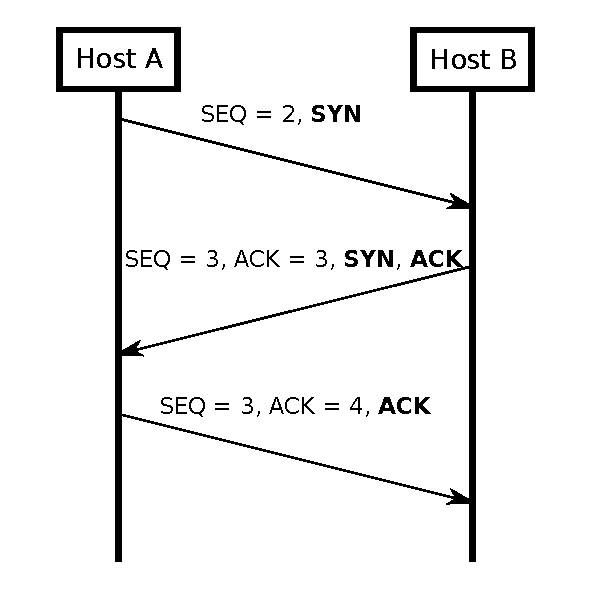
\includegraphics[scale=0.7]{obrazky/prace/SYN_TCP.pdf}
      \end{center}
      \caption[Navázání spojení TCP]{Komunikace mezi hosty při navazování TCP spojení \cite{Jerabek2013}}
      \label{obr:SYN_TCP}
    \end{figure}
 
\par Při výměně dat naznačené na obrázku \ref{obr:TCP} odesílatel každý paket označuje sekvenčním číslem, které je inkrementováno po každém odeslaném paketu. Paket musí být příjemcem označen jako přijatý pomocí paketu obsahující pořadové číslo potvrzovaného paketu a označeného potvrzovacím ACK bitem. Pokud paket není označen jako přijatý je odeslán po vypršení určitého časového rámce opakovaně dokud není potvrzen \cite{Foxc2022}.

    \begin{figure}[!h]
      \begin{center}
        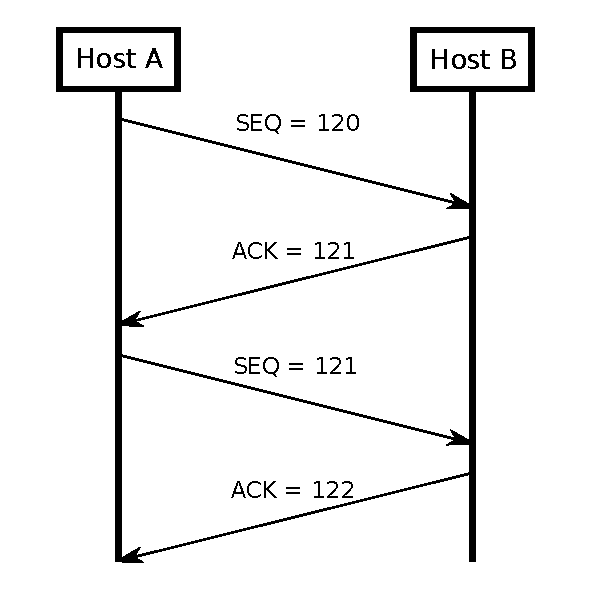
\includegraphics[scale=0.7]{obrazky/prace/TCP_komunikace.pdf}
      \end{center}
      \caption[TCP komunikace]{Jednosměrná TCP komunikace mezi hosty \cite{Jerabek2013}}
      \label{obr:TCP}
    \end{figure}
    
\par Pro ukončení spojení odesílatel vyšle paket s finálním FIN bitem nastaveným na úroveň logické 1. Příjemce potvrdí ukončení spojení pomocí bitů ACK a FIN, odesílatel potvrdí ACK bitem \cite{Foxc2022}. Ukončení TCP spojení si můžeme prohlédnout na obrázku \ref{obr:FIN_TCP}.

    \begin{figure}[!h]
      \begin{center}
        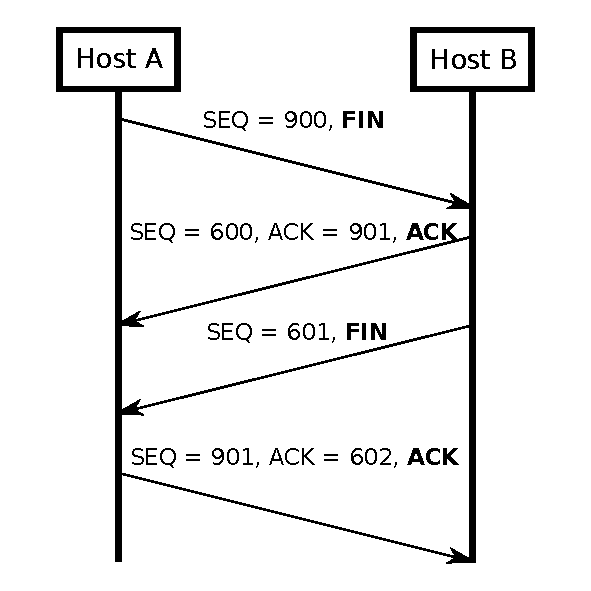
\includegraphics[scale=0.7]{obrazky/prace/FIN_TCP.pdf}
      \end{center}
      \caption[Ukončení spojení TCP]{Ukončení TCP komunikace mezi hosty \cite{Jerabek2013}}
      \label{obr:FIN_TCP}
    \end{figure}
    
\subsection{CoAP}
\par Constrained Application Protocol uveden v standardu RFC 7252 je specializovaný protokol pro přenos dat v sítích IoT. Protokol je založen na REST modelu, kde je server dostupný pod určitou URL adresou a koncová zařízení se na tento server dotazují pomocí GET, PUT, POST a DELETE metod. Díky využití REST modelu je vývoj aplikací využívající CoAP velmi jednoduchý, jelikož vývojáři využívají již známých metod. Pro svou jednoduchost a nízké nároky využívá CoAP jako svou transportní vrstvu protokol UDP, který svým způsobem modifikuje a dovoluje použít základní kontrolu chyb v přenosu. Zpráva CoAP protokolu, vyobrazená v tabulce \ref{table:CoAP}, rozděluje 4 povinné bajty na 2 bity pro verzi indikující verzi CoAP protokolu, 2 bity pro typ zprávy, 4 bity pro délku tokenu a 8 bitů pro kód dotazu či odpovědi. Nastavení typu zprávy ovlivňuje potvrzování zpráv, pro dotazy definuje nutnost či nenutnost potvrzení příjmu dotazové zprávy, pro odpovědi definuje potvrzovací zprávu nebo resetovací zprávu, která potvrzuje příjem dotazu, ale jeho obsah nedokáže server zpracovat. CoAP zpráva by neměla přesahovat maximální velikost jednoho rámce pro zamezení fragmentace paketu \cite{Shelby062014, Bormann20142016, Stusek2019}.
    \begin{table}[!h]
    \caption[CoAP zpráva]{Zpráva protokolu CoAP}
    \label{table:CoAP}
    \begin{center}
    \begin{tabular}{|crcrlrcrlr|}
    \hline
    \multicolumn{1}{|l}{0} & \multicolumn{1}{r|}{1} & \multicolumn{1}{r}{2} & \multicolumn{1}{r|}{3} & 4 & \multicolumn{1}{r|}{7} & \multicolumn{1}{l}{8} & \multicolumn{1}{r|}{15} & 16 & 31 \\
    \hline
    \multicolumn{2}{|c|}{Verze} & \multicolumn{2}{c|}{Typ} & \multicolumn{2}{c|}{Délka tokenu} & \multicolumn{2}{c|}{Kód dotazu/odpovědi} & \multicolumn{2}{c|}{ID zprávy} \\
    \hline
    \multicolumn{10}{|c|}{Token (volitelný)} \\
    \hline
    \multicolumn{10}{|c|}{Možnosti (volitelné)} \\
    \hline
    \multicolumn{6}{|c|}{0xFF} & \multicolumn{4}{c|}{Data (volitelné)} \\
    \hline
    \end{tabular}
    \end{center}
    \end{table}
    
\subsection{MQTT}
\par Message Queuing Telemetry Transport je otevřený komunikační protokol, standardizovaný pod sdružením OASIS, jež implementuje odlehčený publish/subscibe mechanismus pro M2M komunikaci. Protokol MQTT je určen pro zařízení s omezenými zdroji a s omezenou síťovou propustností. Spolehlivou komunikaci zajišťuje transportní TCP vrstva. Varianta MQTTS navíc integruje protokol Transport Layer Security (TLS) pro zajištění autenticity \cite{Xy18NbcqliC08Kok, Stusek2019, Banks2014}. Formát MQTT zprávy si můžeme prohlédnout v tabulce \ref{table:MQTT} 

    \begin{table}[!h]
    \caption[MQTT zpráva]{Zpráva protokolu MQTT}
    \label{table:MQTT}
    \begin{center}
    \begin{tabular}{|cccccccc|}
    \hline
    \multicolumn{1}{|c|}{0} & \multicolumn{1}{c|}{1} & \multicolumn{1}{c|}{2} & \multicolumn{1}{c|}{3} & \multicolumn{1}{c|}{4} & \multicolumn{1}{c|}{5} & \multicolumn{1}{c|}{6} & 7 \\
    \hline
    \multicolumn{4}{|c|}{Typ zprávy} & \multicolumn{1}{c|}{Příznak duplikátu} & \multicolumn{2}{c|}{QoS} & Příznak zachování \\
    \hline
    \multicolumn{8}{|c|}{Zbývající délka} \\
    \hline
    \multicolumn{8}{|c|}{Délka jména topicu MSB} \\
    \hline
    \multicolumn{8}{|c|}{Délka jména topicu LSB} \\
    \hline
    \multicolumn{8}{|c|}{Jméno topicu} \\
    \hline
    \multicolumn{8}{|c|}{ID zprávy MSB} \\
    \hline
    \multicolumn{8}{|c|}{ID zprávy LSB} \\
    \hline
    \multicolumn{8}{|c|}{Zpráva} \\
    \hline
    \end{tabular}
    \end{center}
    \end{table}

\par MQTT infrastruktura je složena ze tří částí a to: publisherem (klient který data odesílá), MQTT brokerem a subscriberem (klient který data přijímá). MQTT broker zajišťuje veškeré funkce MQTT spojení. Udržuje spojení s klienty, zajišťuje Quality of Service (QoS) a základní zabezpečení pomocí autentizace klientů (pokud je povolena). Publisher zasílá zprávy s určitým topicem (tématem, dle kterého můžeme zprávy třídit) na IP adresu MQTT brokera. Pokud nějaký určitý topic chceme sledovat a veškeré zprávy z něj přijímat, registrujeme klienta jako subscribera. Jakmile MQTT brokerovi přijde zpráva s určitým topicem, ihned je odešle všem klientům, kteří tento topic odebírají. \cite{GillisJanuary2021, Stusek2019}. Strukturu MQTT sítě si můžeme prohlédnout na obrázku \ref{obr:MQTT}.

    \begin{figure}[!h]
      \begin{center}
        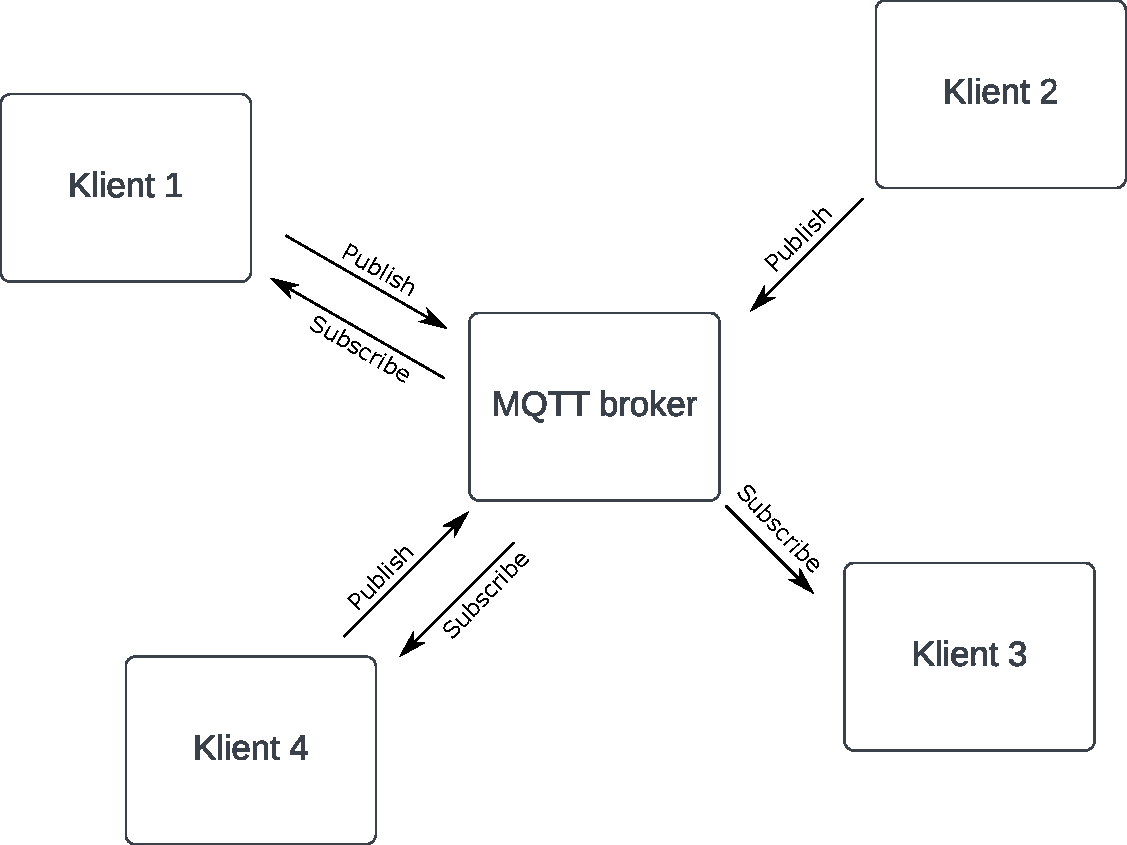
\includegraphics[scale=0.5]{obrazky/prace/MQTT.pdf}
      \end{center}
      \caption[Struktura MQTT sítě]{Struktura MQTT sítě}
      \label{obr:MQTT}
    \end{figure}
    
\par V současné době se můžeme setkat s těmito verzemi MQTT:
    \begin{itemize}
        \item v3.1 vydaný v roce 210 jako první volná verze MQTT, verze je označována jako legacy \cite{lrDVyaBRVfGzwzsO}
        \item v3.1.1 vydána v roce 2014 jako OASIS standard. Mírně modifikuje verzi 3.1 hlavně přidáním session present flagu (informuje klienta o již probíhajícím spojení, klient tak musí pouze začít odbírat určitý topic), povoluje anonymní klienty (anonymnímu klientovy přidá MQTT broker náhodný clientID, funkce je vhodná pro klienty kteří nepotřebují udržovat spojení a zprávy pouze odesílají), přidává podporu okamžitých MQTT zpráv (umožňuje odeslat zprávu bez čekání na potvrzení spojení), zvětšuje velikost clientID (nyní může být až 65535 bajtů dlouhý)a zaručuje že veškeré Stringy budou UTF-8 kódovány \cite{Banks2014}
        \item v5 standardizována v roce 2019 přidala optimalizace pro velké instance, jako vylepšenou autentizaci nebo možnost přidat omezení pro maximální velikost zpráv. Dále zlepšuje verzi v3.1.1 \cite{Liadovc20092022}
    \end{itemize}

\chapter{Hardwarový návrh}
\par Hlavním cílem práce je návrh přesného srážkoměru, který bude možno umístit do terénu bez nutnosti připojení zařízení k elektrickému napájení, je tedy nutné zajistit dostatečnou kapacitu baterie a zvážit použití solárního panelu jenž by podpořil energetickou nezávislost a delší výdrž zařízení. Zařízení by mělo umožňovat real-time odesílání dat.
\par Při výběru vhodného typu srážkoměru jsme se zaměřili na poměr přesnosti, ceny, velikosti a energetické náročnosti. Po zvážení všech zmíněných kritérií jsme zvolili člunkový typ srážkoměru, jež kombinuje dostatečnou přesnost měření srážkových úhrnů s nízkou energetickou náročností. Cena a velikost záleží na výrobci a konkrétním typu člunkového srážkoměru. Pro detekci i malého srážkového úhrnu či rosy, které mohou způsobit útlum signálu vlivem efektu vlhké antény, jsme se rozhodli podpořit srážkoměr dešťovým senzorem. K doplnění informací bude zařízení obsahovat také měření teploty a intenzity světla.
\par Pro zajištění možnosti real-time komunikace jsme se rozhodli pro technologii NB-IoT jelikož operuje v licencovaných pásmech rádiového spektra není omezena střídou mezi vysíláním. Zařízení bude spoléhat na operátora Vodafone, jehož NB-IoT základové stanice poskytují na území České republiky téměř 100 \% pokrytí signálem.
\par Při konečném výběru vhodných elektronických komponent zařízení jsme se řídili parametry uvedenými v datasheetech jednotlivých komponent, u některých komponent také jednoduchými porovnávacími testy. Při výběru jsme museli také zohlednit aktuální situaci na trhu s elektrotechnickými komponenty, která znemožňuje použití určitých součástek z důvodu jejich nedostupnosti. Zjednodušené blokové schéma funkce navrhovaného zařízení je vyobrazeno na obrázku \ref{obr:HardwareBlock}.
    \begin{figure}[!h]
      \begin{center}
        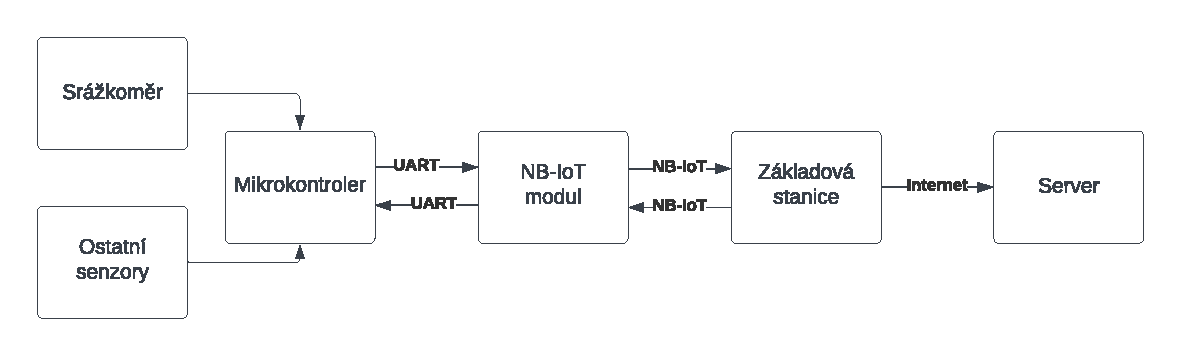
\includegraphics[scale=0.7]{obrazky/prace/HardwareDiagram.pdf}
      \end{center}
      \caption[Blokové schéma - Hardware]{Blokové schéma funkce zařízení}
      \label{obr:HardwareBlock}
    \end{figure}

\section{Espressif Systems ESP32}
\par System on a chip (SoC) ESP32 jsme jako mikrokontroler vybrali z důvodu dostatečného výkonu pro komunikaci s NB modulem, a přitom nízkou energetickou náročnost při hlubokém spánku zařízení, kdy spotřeba modulu klesá na desítky \mikro A. Všechny moduly ESP32 obsahují WiFi konektivitu, která může sloužit pro testování, odesílání dat v případě dostupnosti WiFi sítě nebo pro nahrávání nejnovějších firmwarů pomocí techniky Over The Air (OTA) \cite{UtwRiZcdaaRkidVE}.
\par Pro návrh zařízení v rámci semestrální práce pracujeme s modulem ESP32 WROOM-32E, který se vyznačuje těmito vlastnostmi \cite{UtwRiZcdaaRkidVE}:
    \begin{itemize}
        \item Napájecí napětí 3 až 3,6 V.
        \item ESP32-D0WD-V3 Xtensa dual-core 32bit LX6 mikroprocesor s taktovací frekvencí až 240 MHz.
        \item 448 KB ROM, 520 KB SRAM a 16KB SRAM v Real Time Clock (RTC) části.
        \item IEEE 802.11b/g/n WiFi a Bluetooth v4.2 s podporou Bluethooth Low Energy (BLE), modul WROOM-32E obsahuje integrovanou PCB anténu.
        \item 36x General-purpose input/output (GPIO) pinů podporující:
            \begin{itemize}
                \item 3x hardwarový Universal Asynchronous Receiver-Transmitter (UART)
                \item I2C
                \item čítač pulsů
                \item Analog-to-digital converter (ADC) s rozlišením 12 bitů
                \item Digital-to-analog converter (DAC)
            \end{itemize}
    \end{itemize}

\par Při návrhu výsledného řešení můžeme uvažovat o využití SoC ESP32-S3, nebo ESP32-C3 v pouzdře QFN z důvodu nižší ceny a menší velikosti.

\section{Quectel BC660K-GL}
\par Pro zajištění komunikace po LPWAN NB-IoT byl zvolen modul BC660K-GL od výrobce Quectel. Modul podporuje jak LTE cat. NB1, tak i nejnovější standart LTE cat. NB2, který byl představen ve 14. vydání 3GPP. Výhodou modulu je velmi nízká energetická náročnost v PSM kdy jeho spotřeba klesá dle datasheetu na hodnotu 800 nA, při vysílání v ideálních podmínkách s výkonem 23 dBm = 200mW je udávaná spotřeba 330 mA. Modul je možné napájet v rozsahu 2,2 až 4,3 V. Takto velký napájecí rozsah by dovoloval napájet modul i bez regulátoru napětí. Modul podporuje také značné množství komunikačních protokolů jako: UDP, TCP, MQTT a MQTTS či Lightweight M2M (LwM2M). Mezi podporující rozhraní patří: 2x UART, 4x GPIO, 1x I2C \cite{Xe6siNg2rhN8gnWj}.
\par Ovládání modulu BC660K-GL je zajištěno pomocí AT příkazů pomocí UART linky propojující modul s ESP32. BC660K-GL obsahuje dvě hardwarové UART linky kdy první z nich je použita pro přenos dat při použití modulační rychlosti 115200 Bd/s a pro nahrávání nových verzí firmwaru, pokud je modul v download režimu, při použití modulační rychlosti 921600 Bd/s. Druhá UART linka je určena pro debugging s výchozí modulační rychlostí 6 MBd/s \cite{A41W1voJqm9eaVoi}.
\par V rámci semestrální práce byla použita vývojová deska (devkit) modulu označována jako BC660K-GL-TE-B. Devkit dovoluje komunikovat s modulem pomocí USB počítače po přepnutí přepínače J302 do polohy „MAIN UART TO USB“. Převod mezi USB a UART rozhraním je realizován pomocí USB-UART převodníku od výrobce FTDI umístěného na devkitu. S devkitem můžeme komunikovat také přímo pomocí UART linky mikrokontroleru, pro tuto možnost musíme přepnout přepínač J302 do polohy „MAIN UART TO MCU“. Devkit je vybaven pinoutem kompatibilním s vývojovou platformou Arduino UNO, tohoto pinoutu bylo využito k připojení devkitu k desce plošných spojů, která vznikala v rámci této semestrální práce. Napájení modulu BC660K-GL je zajištěno pomocí 3,3 V regulátoru jehož vývod je připojen k pinu VBAT umístěného na devkitu. Pin VBAT je přímo spojen s napájecím pinem samotného modulu \cite{Ive1rMH0mThtXUvO}.

\section{Použité senzory}
\subsection{Srážkoměr}
\par Jak již bylo zmíněno v úvodu této kapitoly, řešení bude postaveno na člunkovém srážkoměru. Člunkové srážkoměry obsahují magnetický jazýčkový kontakt (ve většině případů zapojený jako NO) spínaný permanentním magnetem umístěném na překlápěcím člunku. Při každém překlopení se magnet dostane do blízkosti jazýčkového kontaktu, který sepne čímž uzavře elektrický obvod. V našem případě sepnutí kontaktu způsobí změnu logického stavu na GPIO pinu mikrokontroleru na úroveň logické 1 (HIGH). Jelikož GPIO pin bude nastaven jako vstupní přerušení (interrupt) způsobí změna logické úrovně volání vlákna programu, který inkrementuje hodnotu $x$. Výsledná hodnota $x$ se po zvoleném časovém úseku převede na odpovídající srážkový úhrn jednoduchou rovnicí $R = x*a$ kde konstanta $a$ představuje definovaný objem překlopení v milimetrech, $R$ představuje srážkový úhrn v milimetrech za nastavený časový úsek (v případě 1 hodiny v mm/h).
\par Jelikož připojení srážkoměru k mikrokontroleru ESP32 bude realizováno pomocí konektoru RJ11 je možné srážkoměry jednoduše měnit. V rámci semestrální práce bude pro testování a tzv. proof of concept použit srážkoměr neznámého výrobce dodávaný k meteostanicím WH1080 a WH1090 jehož výhodou je velmi nízká pořizovací cena (220 Kč\footnote{Dostupný z: \url{https://hadex.cz/t116-srazkomer-k-meteostanicim-wh1080-a-wh1090/}}).

\subsection{Teplotní senzory}
\par Pro zpřesnění měření budou použity dva teplotní senzory jejichž výstupní data se budou mezi sebou průměrovat. Při výběru byli zváženy sensory BME280 od výrobce Bosch a DS18B20 od výrobce Maxim Integrated. 
\par Bosch BME280 je integrovaný obvod pro měření teploty, relativní vlhkosti a atmosférického tlaku. Spotřeba obvodu závisí na požadované přesnosti měření, rychlosti měření a požadovaných veličinách. Typická přesnost měření teplot: ±1 °C, měření relativní vlhkosti: ±3 \%, měření atmosférického tlaku: ±0,25 Pa. Udávaná spotřeba v různých režimech: 
    \begin{itemize}
        \item 0,1 \mikro A v režimu spánku.
        \item 1,8 \mikro A při měření teploty a relativní vlhkosti s obnovovací frekvencí 1 Hz.
        \item 3,6 \mikro A při měření teploty, relativní vlhkosti a atmosférického tlaku při obnovovací frekvenci 1 Hz.
    \end{itemize}
Komunikace mezi mikrokontrolerem a BME280 je umožněna po I2C a SPI sběrnici. Pomocí sběrnice I2C můžeme nativně připojit maximálně dva senzory BME280 a to díky I2C adrese senzoru, která je nastavitelná pomocí pull-up případně pull-down rezistoru na hodnotu 0x77 případně 0x76 \cite{h58i7wDeqx5UV21c}.
\par Maxim Integrated DS18B20 je integrovaný obvod umožňující programovatelné 9 až 12bitové měření teploty. Obvod komunikuje po 1-wire sběrnici umožňující připojení senzoru pouze třemi vodiči (VCC, GND a data). V případě potřeby je možné napájet obvod přímo po datové lince. Na jedné 1-wire sběrnici můžeme mít připojeno několik DS18B20 sensorů, díky unikátnímu 64bitovému identifikátoru, který je každému senzoru při výrobě přiřazen. Rozmezí měřitelné teploty je od -55 °C do +125 °C s udávanou přesností ±0,5 °C (na rozsahu -10 °C až +85 °C). Udávaná spotřeba senzoru při měření je 1 mA, spotřeba v režimu nečinnosti je 750 nA \cite{x3UaJyQqMZRLqJsg}.
\par Pro porovnání stability jsme provedli jednoduchý test, který obsahoval dva senzory BME280, dva sensory DS18B20, senzor DHT22 a interní senzor teploty umístěný uvnitř modulu ESP32 WROOM-32D. Během testu jsme odebíraly vzorky teplot každé dvě minuty (měření senzorem BME280 probíhala ve forced módu, tedy ve stejném módu jako v koncové aplikaci) a výsledky jsme odesílali na server. Zobrazení výsledků probíhalo v prostředí Grafana, kde byly zobrazeny grafy s aktuálními naměřenými daty, s průměrovanými daty za 10 minut a průměr dvou senzorů (DS18B20 a BME280). V první chvíli jsme vyřadili interní senzor teploty modulu ESP32 WROOM-32D\footnote{modul WROOM-32D se od použitého WROOM-32E liší (pro potřeby této práce) pouze ve verzi použitého čipu, moduly jsou v této práci zaměnitelné} jelikož senzor je určen spíše k monitorování teploty jádra v aplikacích se zvýšeným teplem, senzor tak měří teplotu přibližně 50 a více °C. Senzory DS18B20 se od sebe lišili v řádech setin °C, čemuž by odpovídala udávaná přesnost 0,1 °C výrobcem. Senzory BME280 se lišili většinou o 0,3 °C. Při průměrování hodnot ze dvou senzorů se rozdíl hodnot naměřených senzory DS18B20 od hodnot naměřených senzory BME280 pohyboval při nárustu teplot kolem 0,1 °C při poklesu teplot o 0,5 °C. Toto chování si můžeme vysvětlit možnou teplotní setrvačností senzorů DS18B20 jelikož jsme použili voděodolnou variantu senzorů, která je zakončena nerezovou koncovkou. Test byl založen pouze na porovnání senzorů mezi sebou, nebyla testována přesnost senzorů, jelikož výsledky nemůžeme ověřit kalibrovaným teploměrem. Zobrazení výsledků v prostředí grafana si můžeme prohlédnout na obrázku \ref{obr:Grafana}.
\par V semestrální práci jsme se rozhodli použít senzor DS18B20 a to na základě odolnosti (voděodolná varianta) a připojení několika senzorů pomocí jednoho GPIO pinu bez záběru I2C adres.

    \begin{figure}[!h]
      \begin{center}
        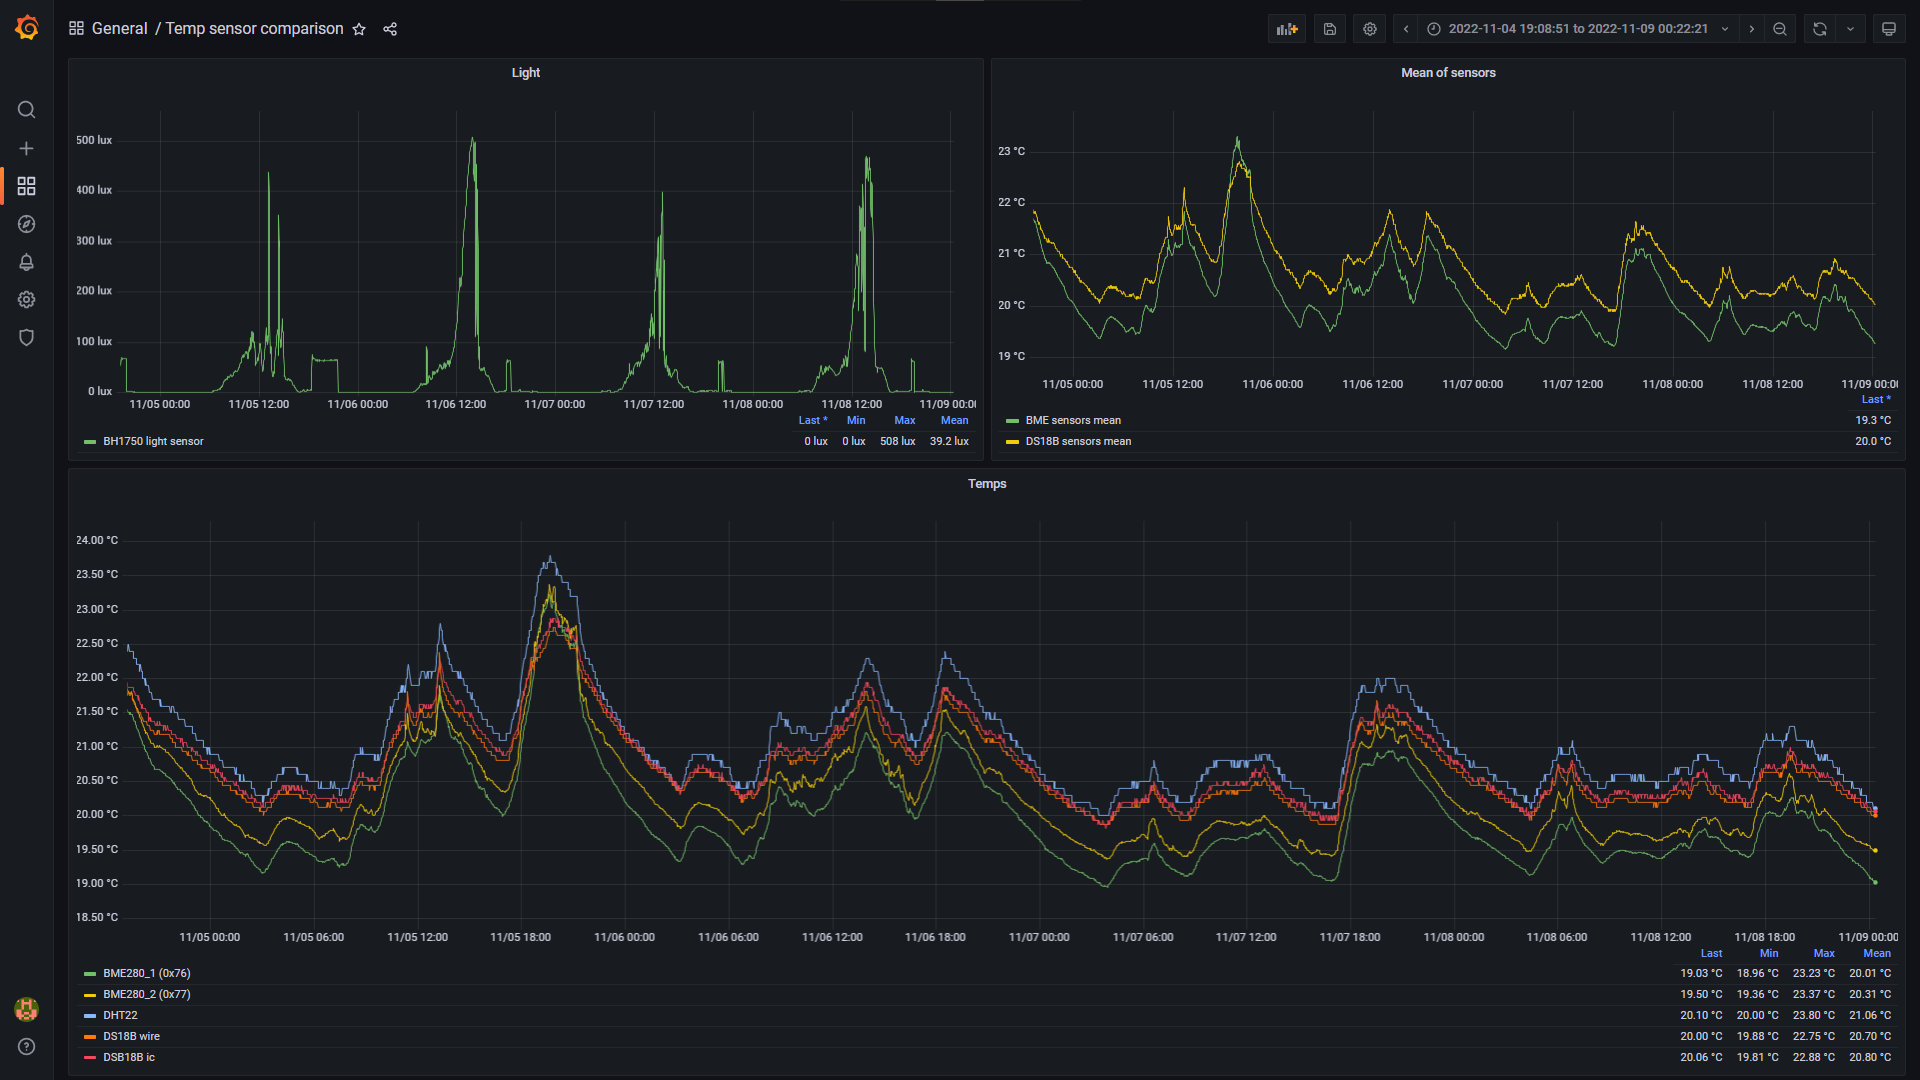
\includegraphics[scale=0.3]{obrazky/prace/Grafana_TempSensor_Coparison_Test.png}
      \end{center}
      \caption[Výsledky testování teplotních senzorů]{Výsledky testování teplotních senzorů v prostředí Grafana}
      \label{obr:Grafana}
    \end{figure}

\subsection{Senzory intenzity osvětlení}
\par Senzory integrující citlivou fotodiodu, analogově digitální převodník a komunikační rozhraní. V rámci semestrální práce používáme senzor BH1750 umístěný na desce plošných spojů (DPS) s vyvedenými piny a osazené nezbytnými součástkami. BH1750 komunikuje po I2C sběrnici, je možné vybrat dvě adresy. Analogově digitální převod má rozlišení 16bitů. Senzor podporuje dva módy rozlišení, a to High o rozlišení 1~lx a Low o rozlišení 4 lx. V případě nižšího rozlišení můžeme dosáhnout rychlejšího měření kdy typický čas potřebný pro odebrání vzorku je 16 ms zatímco v režimu High je to 120 ms. Typická spotřeba senzoru v aktivním stavu je 120 \mikro A \cite{xwYxo72XHkYoFpTN}.
\par Senzorem, který bychom chtěli použít v konečné aplikace je VEML7700 od výrobce Vishay. Jedná se o senzor komunikující po I2C sběrnici, integrující 16bitový analogově digitální převodník. Výhodou oproti senzoru BH1750 je více operačních módů, které ovlivňují spotřebu. Další výhodou je rozlišení 0,0036~lx pro velmi přesné měření. Jelikož VEML7700 není v DIP pouzdře je také vhodnější pro trvalejší montáž ve venkovním prostředí \cite{Schaar20Sep2019}.

\section{Napájení}
\par Napájení počítá s jedno článkovou li-ion (po) baterií s nabíjecím napětím 4,2 V. O~nabíjení článku se stará TP4056, který umožňuje nabíjení článku metodami Constant Voltage (CV) a Constant Current (CC), nabíjecí proud je nastavitelný v několika úrovních od 130 mA až po 1 A pomocí vhodného rezistoru. Nabíjecí obvod je~schopný monitorovat teplotu článku pomocí přídavného termistoru a~v~případě nízké či~vysoké teploty přerušit nabíjení. Maximální vstupní napětí 8~V dovoluje přímé připojení 6~V solárního panelu. Pro nabíjení článku i bez připojeného solárního panelu slouží USB-C konektor. O~ochranu článku se dle verze stará integrovaný obvod DW01A nebo AP9101CK. Oba integrované obvody slouží k~ochraně článku před přepětím, podpětím a zkratem. Použitý typ záleží na aktuální dostupnosti.
\par V řešení využíváme také tzv. „power-path“ jejímž účelem je v případě dostupné energie ze solárního panelu nevyužívat energie uložené v baterii a tím omezit neustálé dobíjení baterie. V případě sepnutí této cesty můžeme též využívat aktivního odvětrávání radiačního štítu, jelikož vestavěný ventilátor je napájen pouze z této cesty, čímž dále šetříme baterii.
\par Monitorování aktuálního nabití baterie je zajištěno pomocí 12bitového A/D převodníku ESP32. Pro snížení maximálního napětí na A/D převodníku je využito napěťového děliče v poměru 1:1.
\par Ve finálním produktu se počítá s držákem baterie 18650 přítomným na DPS.

\section{Testování hardwaru}
\par Po dokončení DPS (na obrázku \ref{obr:Device}) jsme spustili jednoduché testování pro ověření funkčnosti všech komponent. Test se skládal z měření napětí na baterii (ověření napěťového děliče a spínání napájení), měření intenzity osvětlení (ověření funkčnosti I2C sběrnice), měření teploty (ověření oneWire sběrnice a spínnání napájení), simulování srážek (o automatizované spínání obvodu se staral jednoduchý program běžící na mikrokontroleru Espressif ESP8266 umístěného na desce Wemos D1 mini) a odesílání dat na server po síti NB-IoT (ověření funkčnosti UART linky a napájení modulu Quectel BC660K-GL). Zapoejní při testování modulu si můžeme prohlédnout na obrázku \ref{obr:Testing}. Při osazování a následném testování jsme objevili pár chyb v designu a to:
    \begin{itemize}
        \item Chybně zapojený pin na ESP32 pro vstup do režimu stahování firmwaru --- opraveno propojením správného pinu a tlačítka krátkým vodičem.
        \item Chybně orintovaný elektrolitický kondenzátor na vstupu ESP32 --- opraveno otočením kondenzátoru na DPS.
        \item Chybně zapojený jumper pro zapnutí ventilátoru (při propojení do stavu vypnuto by došlo ke zkratovanání VDD33 a GND) --- opraveno neosazením třetího pinu.
        \item Chybně umístěné piny pro napájení development kitu Quectel BC660K-GL-TE-B --- opraveno přidáním napájecích vodičů.
        \item Piny pro připojení baterie jsou na nedostupném místě --- opraveno položením připojovacích pinů.
        \item Popisky umístěné v chybné vrstvě při návrhu DPS, díky čemuž nedošlo k jejich vytisknutí na DPS.
    \end{itemize}

    \begin{figure}[!h]
      \begin{center}
        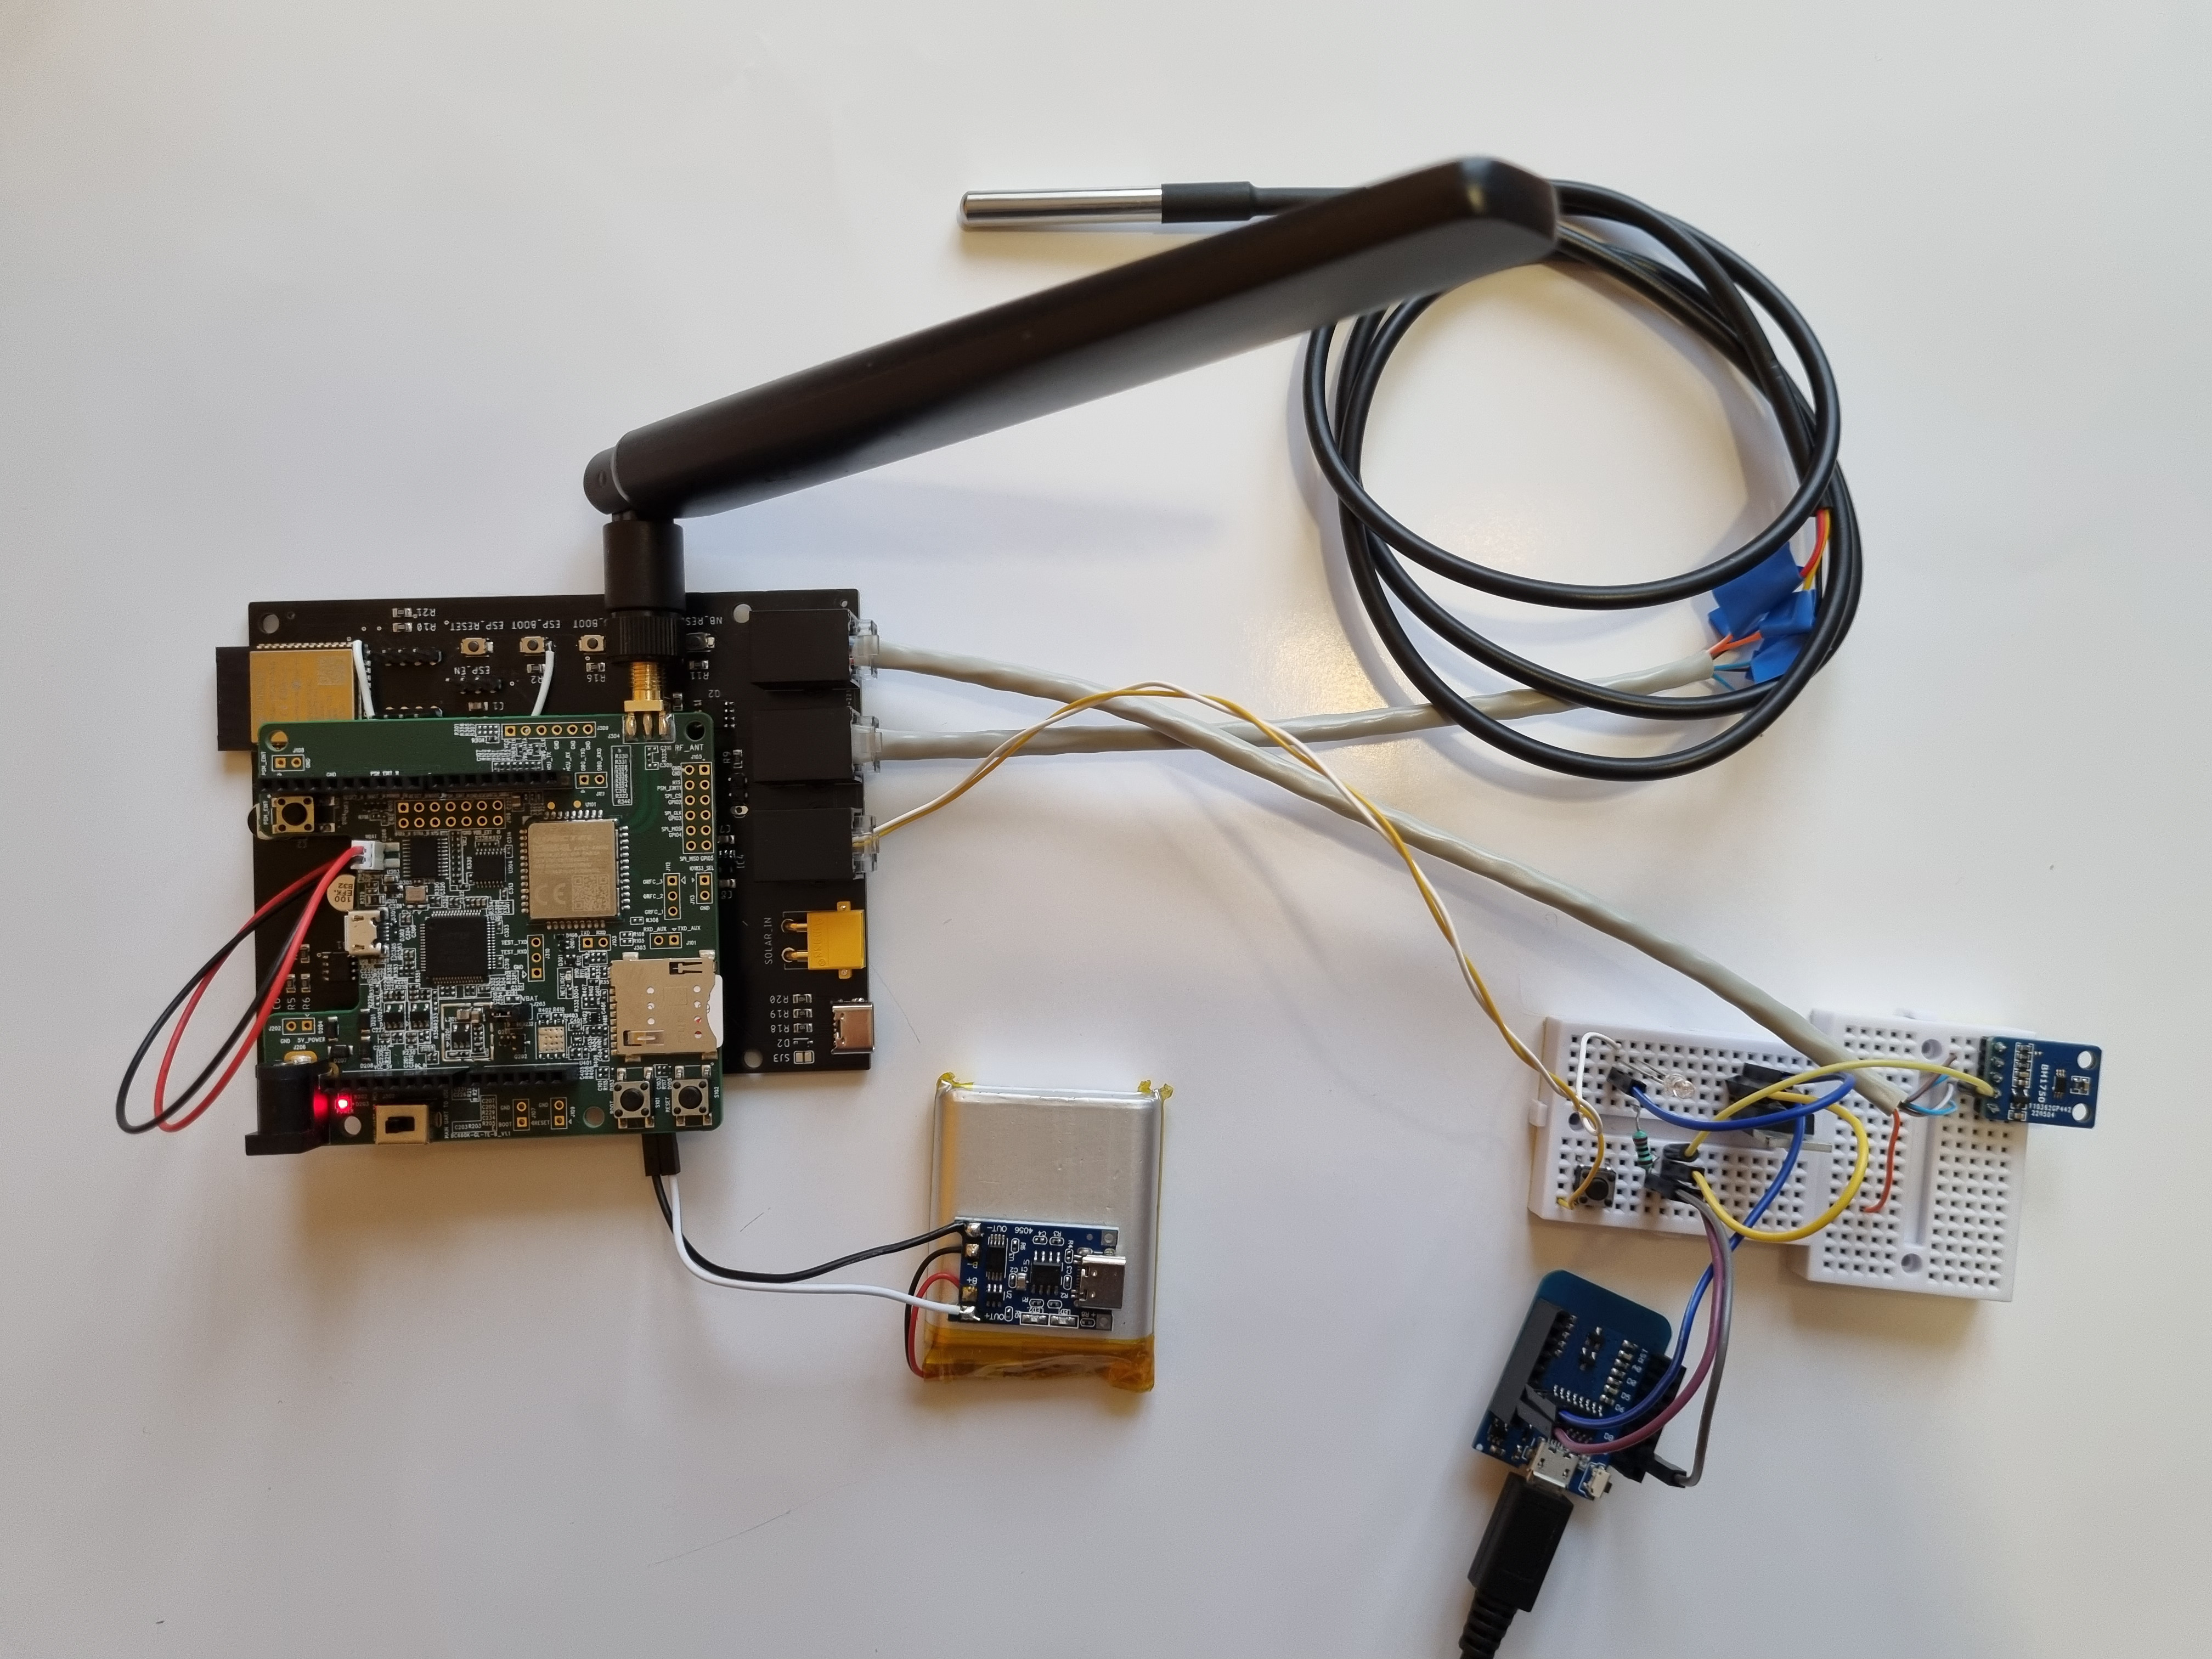
\includegraphics[scale=0.1]{obrazky/prace/Testing.jpg}
      \end{center}
      \caption[Testování zařízení]{Zapojené zařízení při testování}
      \label{obr:Testing}
    \end{figure}

    \begin{figure}[!h]
      \begin{center}
        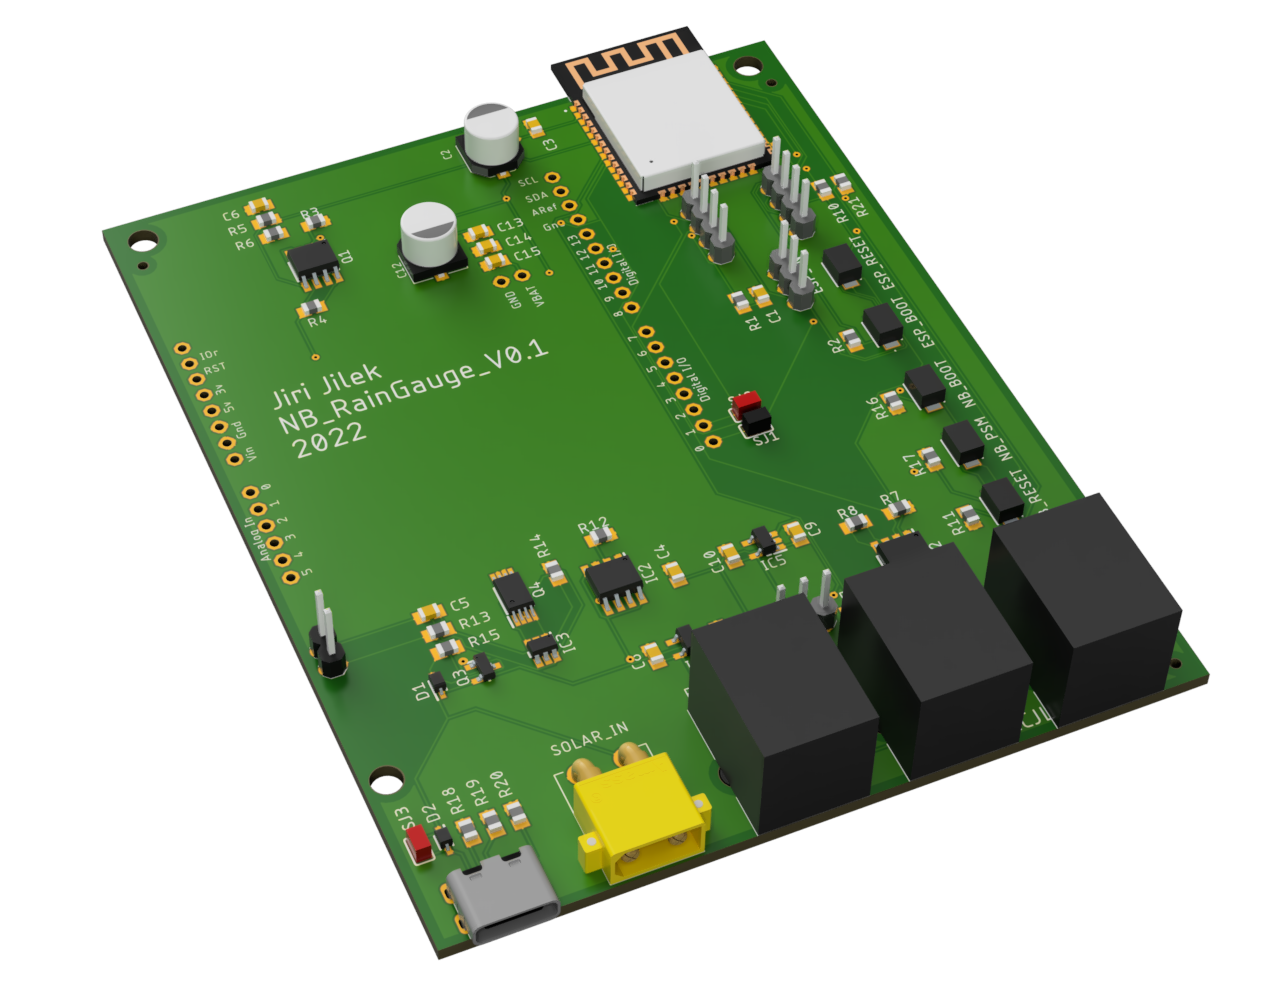
\includegraphics[scale=0.2]{obrazky/prace/Render.PNG}
      \end{center}
      \caption[Render designu DPS]{Render desigu DPS}
      \label{obr:Render}
    \end{figure}

    
    \begin{figure}[!h]
      \begin{center}
        \includegraphics[scale=0.03]{obrazky/prace/Device.jpg}
      \end{center}
      \caption[Podoba zařízení]{Podoba zažízení}
      \label{obr:Device}
    \end{figure}
    




\chapter{Software}
\par Program aplikace vzniknul za pomoci frameworku Arduinu s rozšířením arduino-esp32. Pro práci s AT příkazy nutnými pro komunikaci s NB-IoT modulem využíváme knihovny AT-Command-Library\footnote{Dostupné na Githubu: \url{https://github.com/botletics/AT-Command-Library}}, kterou v rámci forku\footnote{Dotupné na Githubu: \url{https://github.com/R4sp1/AT-Command-Library}} dále rozšiřujeme pro potřeby modulu Quectel BC660K-GL. Knihovna v momentální fázi implementuje řešení pro kontrolu odpovědi NB-IoT modulu na zadaný příkaz a probouzení modulu pomocí pinu PSM\_EINT\_N. Algoritmus, kterým se zařízení řídí při běhu programu je znázorněn na obrázku \ref{obr:Software}. V základu se běh programu řídí na základě dvou podmínek – „Došlo k probuzení zařízení díky překlopení srážkoměru?“ a „Je čas odeslat data?“. Pokud dojde k probuzení zařízení na základě překlopení srážkoměru, zařízení tuto událost uloží do paměti a porovná čas probuzení s časem odeslání dat. Pokud je čas probuzení menší, zařízení upraví dobu spánku, aby došlo k odeslání dat přibližně ve stanovenou dobu. Pokud je čas odeslání dat, zařízení probudí veškeré senzory, přijme jimi naměřená data a data pomocí NB-IoT modulu odešle na server. Na základě nastaveného intervalu mezi odesíláním dat se do paměti zařízení uloží čas dalšího odeslání dat a zařízení přejde do hlubokého spánku, tak aby se v určený čas probralo. Veškerá data, které zařízení ukládá pro potřeby běhu programu (počet překlopení srážkoměru a čas dalšího odeslání dat) je uložen v RAM paměti nacházející se v RTC části modulu ESP32, tato část zůstává napájena i během hlubokého spánku a nedojde tak k resetování této paměti. Paměť je resetována pouze v případě restartu zařízení.

    \begin{figure}[!h]
      \begin{center}
        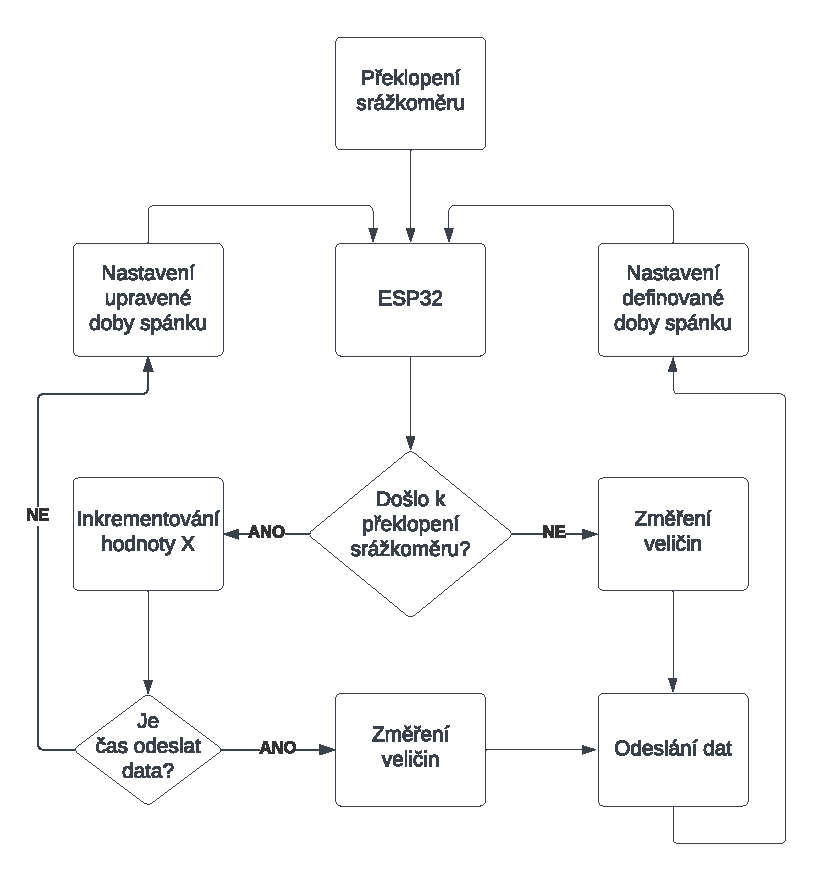
\includegraphics[scale=1]{obrazky/prace/SoftwareDiagram.pdf}
      \end{center}
      \caption[Algoritmus]{Algoritmus programu}
      \label{obr:Software}
    \end{figure}

\section{Aplikace na serveru}
\subsection{Zpracování dat}
\par Zpracování dat probíhá v open source frameworku Node-RED vytvořeném společností IBM pro propojení zařízení a aplikací v IoT projektech. Node-RED je navrhnut pro vytváření JavaScript funkcí na základě spojování rozhodovacích bloků s minimem psaného kódu. V našem případě je Node-RED připojen k MQTT brokerovy jako Subscriber a odebírá určitý topic. Po přijetí MQTT zprávy jsou data v ní obsažena zpracována a následně uložena do databáze, která je také do Node-RED připojena.

\subsection{Databáze}
\par Time series database (TSDB) je optimalizovaný databázový systém pro ukládání dat, které se mění s čase. TSDB mají implementovány mechanismy pro ukládání dat označených časovým razítkem, mechanismy pro kompresy těchto dat, mechanismy pro sumarizaci těchto dat a mechanismy pro získávání dat pomocí časových rozmezí. U časově závislých dat je často zásadní ukládání velmi přesných dat, která jsou objemově často velmi velká. Po určitém čase již ale není potřeba data nadále uchovávat s takovouto přesností, a tak je zvolen ideální kompromis mezi objemem dat a přesností, data v tento moment můžeme například za určitý časový úsek průměrovat či sčítat a uložit pouze výsledek těchto operací \cite{2oiqkV8OrCVn718j}. 
\par V naší práci pracujeme s InfluxDB 2.0, který v jednom balíčku integruje TSDB InfluxDB, Chronograf pro zobrazování dat z databáze InfluxDB a Kapacitor, který zpracovává data z InfluxDB (odesílá upozornění, aplikuje uživatelské funkce).


\subsection{Zobrazení dat}
\par Vzhledem k použití balíčku InfluxDB 2.0, který obsahuje modul pro přímé zobrazení dat z databáze, není přímo nutné využívat další software pro zobrazení dat. Nicméně vizualizační nástroj Grafana je svojí přizpůsobitelností a rozšiřitelnosti defacto standart pro vizualizaci dat z různých zdrojů dat. S modulem „Panel“ můžeme zobrazit data z databází přímo či po jejich úpravě pomocí matematických funkcí v různých vizualizačních stylech (graf, tabulka, log). Pro vytváření upozornění můžeme využít modulu „Alerts“, který dovoluje pokročilé nastavení mezních hodnot pro odeslání upozornění nebo správu již aktivních upozornění. Pro lepší prezentaci můžeme data také anotovat či vizualizovat v dalších stylech pomocí široké palety uživatelských modulů, které je možné do nástroje Grafana doinstalovat. Výsledný dashboard, obsahující všechny nastavené panely, můžeme snadno zobrazovat, vkládat do webových stránek nebo sdílet.

\begin{figure}[!h]
      \begin{center}
        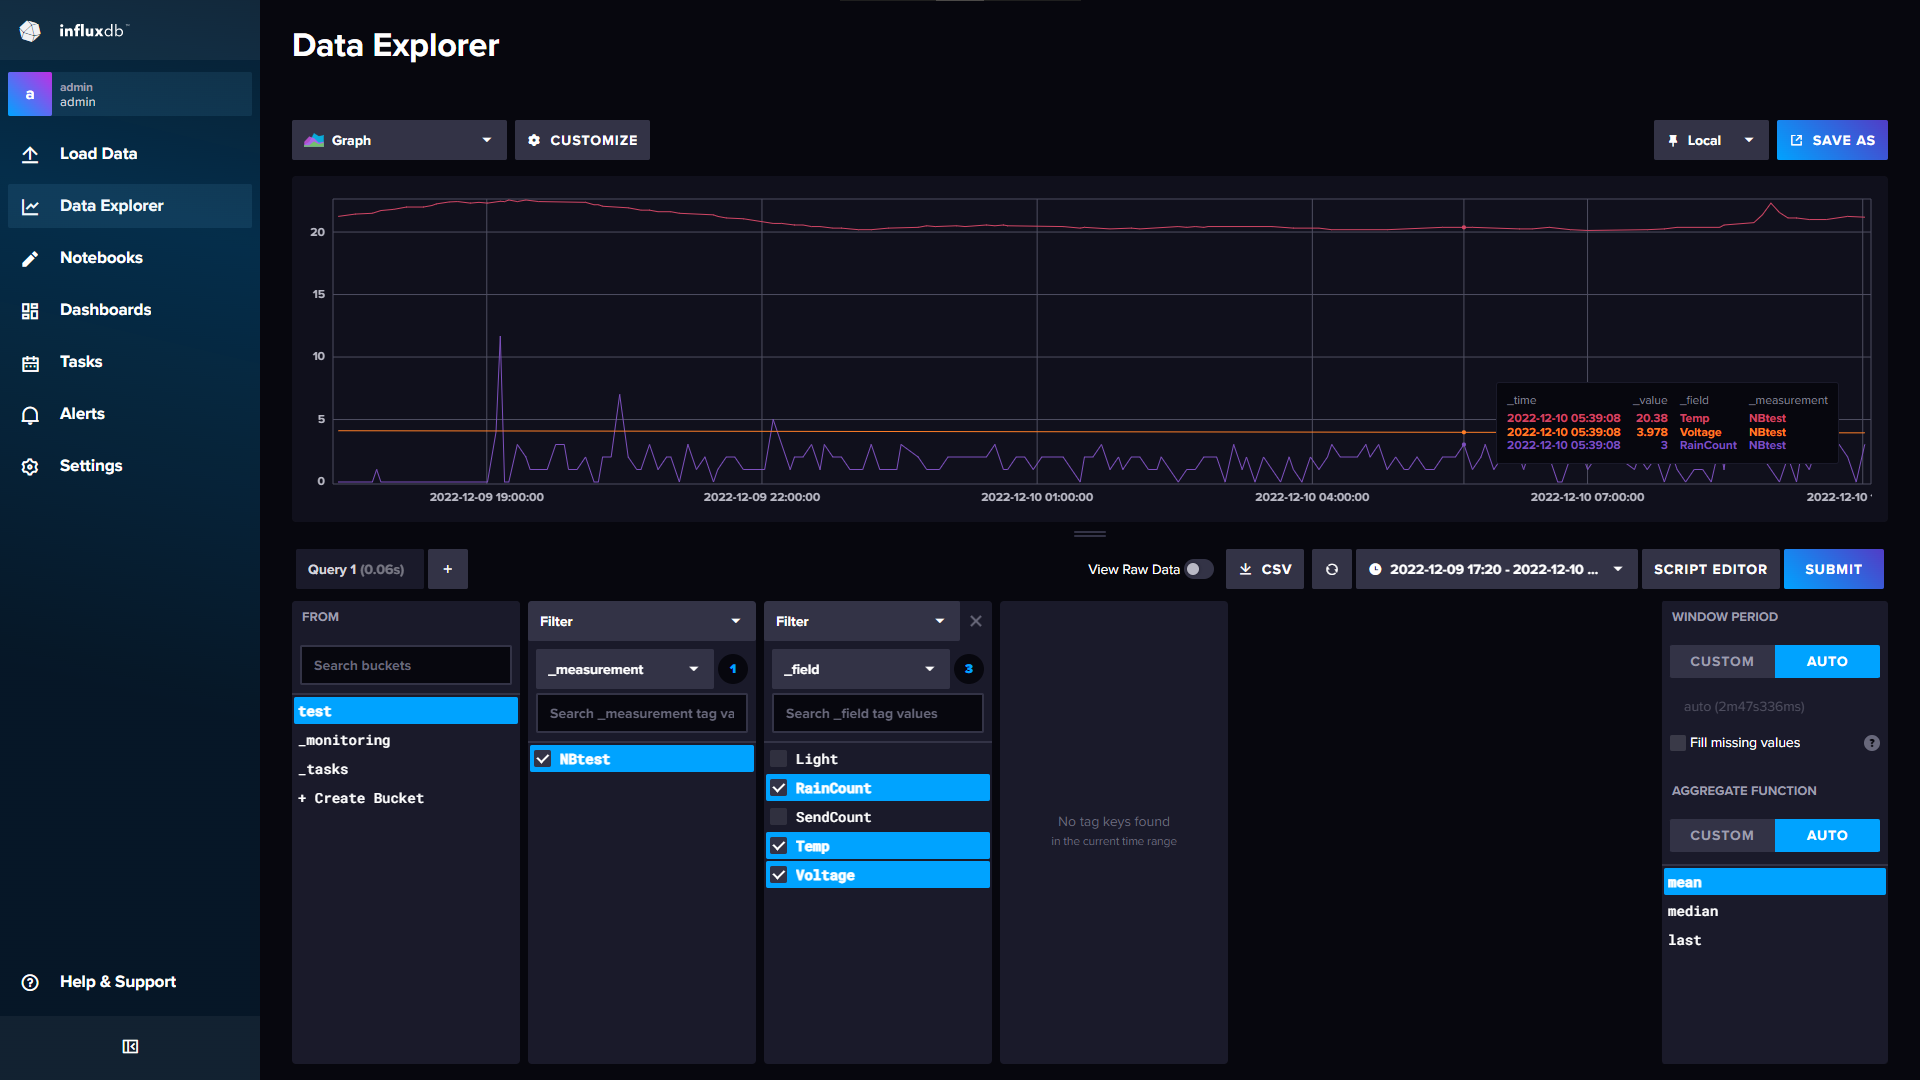
\includegraphics[scale=0.3]{obrazky/prace/Influx_Test.png}
      \end{center}
      \caption[Data z testování]{Data z testování zobrazena v prostředí InfluxDB 2.0}
      \label{obr:Influx}
    \end{figure}